\chapter{Рухальная актыўнасьць}

\section{«Маларухомы» мозг}

Уявім сабе тыповы лад жыцьця сучаснага гарадзкога чалавека: раніцай гараджанін устае, едзе на працу, дзе праводзіць седзячы за сталом восем гадзінаў, адцягваючыся на каву і абед, затым едзе назад дадому, таксама седзячы, бавіць час у~фатэлі перад экранам ці зь сябрамі за сталом. У лепшым выпадку пару разоў на тыдзень ходзіць у~сілоўню і, магчыма, пагуляць у~парк на выхадных. Стамляючыся ад сядзеньня, аддае перавагу адпачынку на канапе напаўлежачы. 

\textbf{Гэта~--- маларухомы, сядзячы лад жыцьця, пагроза здароўю і самаадчуваньню, прычына нізкай энэргічнасьці. Чым меней мы трацім энэргіі, тым болей стомленымі пачуваемся.}

Праблема ўласна ў~сядзеньні: атрымліваецца, што больш за дзесяць гадзінаў на дзень чалавек сядзіць, і гэта прыводзіць да безьлічы неспрыяльных праяваў, у~тым ліку і не зьвязаных зь лішняй вагой: болі ў~сьпіне, артэрыяльная гіпэртэнзія, гемарой, дэпрэсія і многае іншае.

Цяпер уявім чалавека, які жыве па падобным графіку, але ўключае ў~свой лад жыцьця больш руху: робіць з~раніцы зарадку, на працу едзе роварам або выходзіць на прыпынак раней, каб прайсьціся пешшу, карыстаецца лесьвіцай замест ліфта, ходзіць, размаўляючы па тэлефоне, частку працы робіць стоячы, сустракаецца зь сябрамі за тэнісам ці прабежкай, трымае дома гіру, каб раз на дзень бадзёра яе пакідаць, можа глядзець серыял на велатрэнажоры, любіць адпачываць актыўна. 

\textbf{Гэта~--- актыўны лад жыцьця, абарона здароўя, крыніца энэргіі і матывацыі кожны дзень.}

Ня варта прыдумляць, што для руху ў~нас няма часу. Мы нарадзіліся для руху і можам паўнавартасна жыць, рухаючыся больш. Як слушна кажуць, практыкаваньні могуць замяніць шмат лекаў, але ніводны зь іх не заменіць практыкаваньняў.

\emph{Паглядзіце на сябе ў~люстэрка: вы можаце ўбачыць, як фізычная актыўнасьць зьмяніла нас у~працэсе эвалюцыі. На нашым целе ёсьць некалькі дзясяткаў прыкметаў, напрыклад, доўгія ногі, адсутнасьць футра, пашыраныя потавыя залозы, вузкая талія, якая дазваляе махаць рукамі пры бегу, вялікія ягадзічныя цягліцы, форма чэрапа, астуджальная кроў (у жывёлаў сыстэма астуджэньня працуе горш), патылічная зьвязка, якая стабілізуе галаву, невялікая пятавіца (пятавая косьць), адмысловае ўладкаваньне элястычных зьвязкаў~--- усё гэта прынады для трывушчасьці пры бегу. Каля двух мільёнаў гадоў таму нашы продкі маглі бегма на доўгай дыстанцыі загнаць жывёлаў да зьнясіленьня і так палявалі. Таму нашае цела ідэальна прыстасаванае для працяглага бегу.}

З фізычнай актыўнасьцю шчыльна зьвязаныя многія органы і сыстэмы, у~тым ліку мэтабалізм і функцыянаваньне галаўнога мозгу. Мы проста створаныя для руху: 80\,\% нашага цела і 80\,\% мозгу «працуюць на рух», а~40\,\% цела~--- гэта цягліцы.

\textbf{У працэсе эвалюцыі ішоў адбор на трывушчасьць і рухомасьць; той, хто ня рухаўся,~--- гінуў.} Цывілізацыя прынесла нам магчымасьць перасоўвацца на тысячы кілямэтраў, пры гэтым мы рухаемся ўсё менш і менш. Грамадзкі і асабісты транспарт, цягнікі, самалёты~--- усё гэта скарачае нашу рухальную актыўнасьць. Замест карыстаньня лесьвіцамі мы езьдзім на ліфтах, а~рост насельніцтва ў~гарадах прывёў да таго, што вуліца становіцца загазаваным, шумным і небясьпечным месцам, што, натуральна, зьмяншае наша жаданьне персоўвацца па ёй пешшу.

Наша праца стала амаль цалкам разумовай~--- ня толькі ў~офісе, але й дома. Мы купляем ежу, якую нам прывозіць кур'ер, посуд мые пасудамыйная машына, адзеньне мые пральная машына, прыбірае робат-пыласос. Шмат часу мы бавім не на вуліцы, а~ў памяшканьнях, дзе заўсёды ёсьць магчымасьць прысесьці. 

\infobox{Наша культура вучыць, што «ў нагах праўды няма», а~выхаваньне дзяцей спыняе высокі ўзровень актыўнасьці і гульні, прымушае сядзець ціха і абмяжоўваць рухі. Так наш мозг прывучаецца да таго, што трэба паводзіцца скавана, нерухома, і робіцца «маларухомым».}

У сярэднім 30--50\,\% людзей вядуць маларухомы лад жыцьця, а~яшчэ 20--40\,\% хоць і рухаюцца больш, але гэтага ўсё роўна недастаткова для падтрыманьня аптымальнага здароўя. Рух~--- гэта натуральная чалавечая патрэба, такая ж, як патрэба ў~ежы, вадзе, бясьпецы або інтэрнэце. Многія людзі недаацэньваюць пагрозу дэфіцыту фізычнае актыўнасьці, прытым што менавіта адсутнасьць руху зьяўляецца адной зь вядучых прычынаў неінфэкцыйнай хворнасьці і пашкоджвае практычна ўсе органы і сыстэмы арганізма.

\textbf{Фізычная дэтрэнаванасьць}~--- гэта чыньнік рызыкі заўчаснага старэньня. Стан нашых цягліцаў шмат у~чым вызначае наш біялягічны ўзрост. Як гаворыцца ў~анекдоце: «Трэнэр сказаў, што спорт дадасьць мне некалькі гадоў жыцьця, і гэта праўда. Я зрабіў 10 адцісканьняў, і па адчуваньнях мне 85». \textbf{Чым ніжэйшая ваша трывушчасьць, тым вы сапраўды «старэйшыя». Слабы~--- значыць, стары. Моцны~--- значыць, малады, незалежна ад вашага пашпартнага ўзросту. Станавіцеся мацнейшымі!}

Дэфіцыт руху~--- гэта чацьвёрты па значнасьці чыньнік рызыкі сьмерці: кожны трэці дарослы ў~сьвеце рухаецца недастаткова і 9\,\% усіх заўчасных сьмерцяў у~сьвеце зьвязаныя менавіта зь недахопам руху. Яшчэ са школьных часоў, калі дзеці з~хваробай вызваляліся ад фізкультуры, існуе міт: калі вы захварэлі, то найлепшым выйсьцем будзе ляжаць і меней рухацца. Гэта ня так. Рухацца важна ня толькі для зьніжэньня рызыкі захворваньняў, але й хворым людзям.

\emph{Напрыклад, нават пры ракавых захворваньнях сілавыя трэніроўкі дазваляюць як захаваць, так і павялічыць цяглічную масу, лягчэй пераносіць хіміятэрапію, палепшыць зыходы. Раней лекары забаранялі рухацца і пасьля праблемаў з~сэрцам, і пры расьсеянным склерозе. Цяпер жа даведзена, што раньняя рухальная рэабілітацыя дапамагае пры хваробах сэрца, а~пры расьсеянным склерозе нават запавольвае разьвіцьцё хваробы.}

\subsection*{Пытаньні і заданьні}

1. Наколькі энэргічным вы выглядаеце і пачуваецеся?

2. Якімі відамі спорту або актыўнасьці вы захапляецеся?

3. Ці «сядзячы» ў~вас мозг? У сытуацыях чаканьня вы адразу шукаеце крэсла ці гатовыя пастаяць?


\section{Здароўе і рух}

«Як суконшчыкі чысьцяць сукны, выбіваючы іх ад пылу, так і гімнастыка чысьціць арганізм»,~--- словы Гіпакрата, а~яму можна верыць. Сапраўды, рух стымулюе аўтафагію~--- самаачышчэньне клетак. 

\infobox{Жыцьцё~--- гэта рух, і калі руху становіцца менш, то становіцца менш і жыцьця.}

\begin{figure*}[htb!]
  \centering
  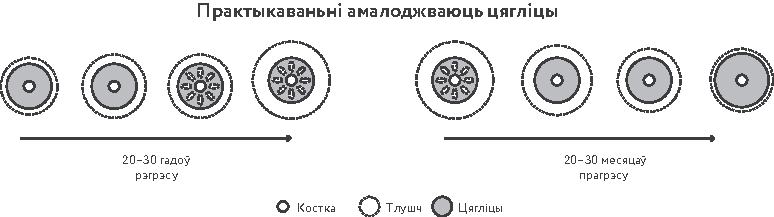
\includegraphics[scale=1.2]{willpower/ch5/1.pdf}
\end{figure*}

Гэта такое замкнёнае кола: чым больш мы фізычна актыўныя, тым лягчэй нам падтрымліваць гэтую самую актыўнасьць. Апроч іншага, практыкаваньні важныя для падтрыманьня дастатковай цяглічнай масы: у~сярэднім з~35 гадоў пачынае адбывацца паступовая страта цяглічнай масы, якая з~узростам толькі ўзмацняецца (саркапэнія), і цягліцы замяшчаюцца тлушчам.

Размаўляючы з~многімі людзьмі, я дзіўлюся, наколькі мы недаацэньваем важнасьць руху і пераацэньваем важнасьць спорту. Рух ня толькі для таго, каб напампоўвацца, рух уплывае на ўсе сфэры жыцьця~--- ад упэўненасьці ў~сабе, кантролю апэтыту, паляпшэньня працы мозгу і шматлікага іншага. Фізычная актыўнасьць~--- гэта яшчэ і прывабнасьць і сэксуальнасьць за кошт кантролю вагі, лепшай структуры цела і выдатнага цяглічнага тонусу.

Рэч ня толькі ў~колькасьці, але і ў~якасьці цягліцаў. «Гультаяватыя» цягліцы горш спальваюць тлушчы, а~вось фізычная актыўнасьць зьмяняе мэтабалізм цягліцаў, амалоджвае іх, павялічвае ў~іх колькасьць мітахондрый, павялічвае іх актыўнасьць. Такія «актыўныя» цягліцы лепш спальваюць тлушчы, выдзяляюць больш чыньнікаў росту, абараняюць ад лішку глюкозы і тлушчу ў~крыві пры стрэсе. Таму не хвалюйцеся, што цягліцы не растуць,~--- яны проста пачынаюць працаваць нашмат лепш.

\subsection*{Мэтабалізм}

Цягліцы важныя ня толькі для руху, яны таксама зьяўляюцца магутнай абаронай мэтабалізму. Фізычная актыўнасьць і цяглічны тонус зьмяншаюць рызыку атлусьценьня і цукроўкі, павялічваюць адчувальнасьць да інсуліну. Цяпер, калі я пішу гэтыя радкі, мільёны людзей па ўсім сьвеце замкнёныя ў~дамах на карантын. \textbf{Адыліж часта мы зусім добраахвотна замыкаем самі сябе.}

\emph{Актыўнасьць меншая за 1000 крокаў на дзень за паўмесяца ў~людзей зь пераддыябэтам выклікае моцнае пагаршэньне вугляводнага абмену. Умераныя сілавыя трэніроўкі ўсяго два разы на тыдзень аднаўляюць адчувальнасьць да глюкозы ў~кожнага трэцяга ў~гэтай жа групе людзей.}

\subsection*{Сэрца}

Фізычная актыўнасьць павялічвае элястычнасьць сасудаў, паляпшае працу сэрца, спрыяе выдзяленьню рэчываў, якія расслабляюць сасуды і паляпшаюць крывацёк. 

\emph{У прадстаўнікоў плямёнаў паляўнічых-зьбіральнікаў нават з~узростам не адбываецца прыкметнага павелічэньня артэрыяльнай гіпэртэнзіі. Чаму? Таму што іх звычайная паўсядзённая актыўнасьць, такая як хада пешшу, зьмена паставы, сядзеньне на кукішках, у~14 (!) разоў большая, чым у~эўрапейцаў. Чыньнік сонца, якое таксама зьмяншае ціск, таксама грае сваю ролю.}

\begin{figure}[htb!]
  \centering
  
\includegraphics[scale=1.5]{willpower/ch5/2.pdf}
\end{figure}

Пры любой актыўнасьці выдзяляецца аксід азоту NO~--- ён ня толькі зьніжае ціск, але і пашырае сасуды, запавольвае працэсы старэньня, паляпшае працу мітахондрый, памяншае акісьляльны стрэс, важны для імунітэту. У мужчынаў першымі часта пакутуюць сасуды чэлеса, а~эрэктыльныя парушэньні ў~два разы павялічваюць імавернасьць ня толькі інфаркту, інсульту, але і на 33\,\% павялічваюць рызыку раньняй сьмерці. Ужо калі вам пляваць на вашыя цягліцы, няўжо вам напляваць і на сваю эрэкцыю?

\subsection*{Батанік ці мацак?}

Напэўна кожны чуў показкі пра разумнага, але кволага «батаніка» і дурнога, але дужага «мацака». У рэальнасьці гэта хутчэй выключэньне, чым правіла. Даведзена, што чым вышэйшы ў~дзіцяці ўзровень актыўнасьці і чым лепш у~яго разьвітыя цягліцы, тым больш эфэктыўна яно праходзіць тэсты на памяць, можа лягчэй засяродзіцца і лепей вучыцца.

Зрэшты, ніколі ня позна пачаць займацца спортам. У дарослых людзей розныя віды актыўнасьці паляпшаюць розныя мазгавыя функцыі: сілавыя трэніроўкі ўплываюць на выканаўчыя функцыі і асацыятыўную памяць, аэробныя~--- на вербальную памяць, бег басанож або лазаньне па дрэвах~--- апэратыўную памяць.

\emph{У пажылых людзей 45-хвілінны шпацыр хуткім крокам тры разы на тыдзень можа павялічыць аб'ём гіпакампа на 2--3\,\%. Гучыць ня вельмі натхняльна, але гэтага дастаткова, каб зь лішкам перакрыць узроставае паніжэньне яго аб'ёму.}

Як казаў Ніцшэ, «не давярай аніводнай думцы, якая нарадзілася ў~нерухомасьці». Рух пачынаецца з~актыўнасьці нэўронаў, і вельмі многія структуры мозгу так ці інакш зьвязаныя з~рухам. Таму фізычная актыўнасьць крытычна важная як для мазгавой прадуктыўнасьці, так і для прафіляктыкі нэўрадэгенэратыўных захворваньняў. Дастаткова рухаючыся, мы зьніжаем выяўленасьць дэпрэсіі ды павышаем выпрацоўку асаблівага нэўратрафічнага чыньніка мозгу BDNF, які павялічвае нэўраплястычнасьць.

\begin{figure}[htb!]
  \centering
  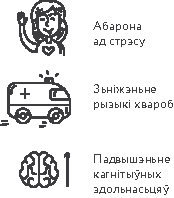
\includegraphics[scale=1.5]{willpower/ch5/3.pdf}
\end{figure}

\emph{Далёка ня ўсе віды актыўнасьці стымулююць моцнае выдзяленьне чыньніку росту нэўронаў і гліяльных клетак, напрыклад расьцяжка аказалася неэфэктыўная, а~вось бег і сілавыя віды спорту выдатна дапамагаюць «паразумнець». Таму я не лічу ёгу і расьцяжку адэкватнай заменай фізычнай актыўнасьці.}

Фізычная актыўнасьць запавольвае старэньне і значна паляпшае якасьць жыцьця ў~старасьці: на 20\,\% паляпшае якасьць жыцьця, аддаляе непрацаздольнасьць і можа падаўжаць пэрыяд здароўя на цэлых 15 гадоў! Пры гэтым розныя віды спорту падаўжаюць жыцьцё ад 3 да 6 гадоў. Акрамя таго, дастатковы ўзровень руху на 11\,\% зьмяншае сьмяротнасьць ад ракавых хваробаў: анкалягічныя хворыя, якія займаюцца фізычнай актыўнасьцю, маюць лепшыя зыходы.

\subsection*{Рухальная актыўнасьць і стрэс}

Натуральная рэакцыя на стрэсары~--- «біць або бегчы», таму актыўнасьць дапамагае бясьпечна ўтылізаваць мэтабалічныя стрэсавыя эфэкты і выкарыстоўваць «па прызначэньні» стрэсавы выкід тлушчаў і глюкозы ў~кроў. Фізычная актыўнасьць ня толькі зьніжае картызол, але й дапамагае падтрымліваць аптымальны ўзровень тэстастэрону, які «падае» пры стрэсе. Чым больш вы натрэніраваныя фізычна, тым больш стрэсаўстойлівыя і стрыманыя на перамовах: невыпадкова многія палітыкі і бізнэсмэны актыўна займаюцца спортам, а~многія спартоўцы пасьпяховыя ў~бізнэсе і палітыцы. 

\textbf{Сярэдняй актыўнасьці недастаткова: у~людзей, якія рухаюцца «ўмерана», рызыка дэпрэсіі на 25\,\% вышэйшая ў~параўнаньні з~тымі, хто актыўна займаецца спортам.}

\textbf{Аздаравіце свае гены.} Фізычная актыўнасьць аздараўляе ня толькі звонку, але і знутры: зьніжае ўзровень хранічнага запаленьня, а~таксама актывуе многія карысныя для здароўя гены і рэгулятарныя каскады, напрыклад AMPK, што зьніжае залішнюю «дзейнасьць» ужо вядомага нам mTOR і стымулюе аўтафагію.

\emph{У адным з~дасьледаваньняў менавіта фізычная актыўнасьць змагла павысіць экспрэсію некалькіх сотняў ахоўных генаў. Іншыя навукоўцы вывучалі эпігенэтычны ўплыў спорту на актыўнасьць генаў: удзельнікаў прымушалі круціць пэдалі велатрэнажора адной нагой цэлыя тры месяцы. Дзіўнае заданьне, але яно дапамагло выключыць уплыў іншых чыньнікаў. Высьветлілася, што цягліцы на назе зьмяніліся ў~пяці тысячах пунктаў, акрамя таго спорт уплываў на актыўнасьць 175 генаў у~клетках сэрца, прымушаючы іх больш актыўна аднаўляцца і расьці.}

\textbf{Актыўнасьць~--- гэта сапраўдны лек.} Тыя, хто яго не прымае, мае рызыку зьяўленьня хваробаў сэрца на 45\,\% вышэй, астэапарозу~--- на 59\,\%, дыябэту~--- на 50\,\%. Спорт памяншае рызыку разьвіцьця больш за 15 відаў раку: кішачніка, малочнай залозы, эндамэтрыя, нырак, печані, стрававода, лёгкіх, страўніка, маткі, лімфомы, міеламы. Пры гэтым для многіх відаў раку ступень зьніжэньня рызыкі была дозазалежнай, то бок больш спорту~--- менш рызыка. Вядома, занадта захапляцца бегам пад пякучым сонцам ня трэба: у~дасьледаваньні выявілі павелічэньне рызыкі разьвіцьця мэляномы пры павышэньні актыўнасьці. Актыўнасьць паляпшае шматлікія біямаркеры: зьмяншаюцца паказьнікі запаленьня, мачавой кіслаты, ціску, глікаванага гемаглабіну. Можа нават памяншацца таўшчыня комплексу інтым-мэдыя, што гаворыць пра адваротнае разьвіцьцё атэрасклерозу.

\infobox{Чым даўжэй вы трэніруецеся, тым больш прыкметна нарастае розьніца паміж вамі і тымі, хто ляжыць на канапе, менавіта ў~разрэзе рызыкі для здароўя. І наадварот: калі вы рухаецеся менш, усе гэтыя лічбы працуюць супраць вас.}

\textbf{Гіпадынамія} павялічвае рызыку інфаркту ў~два разы, сьмяротнасьці ад яго~--- у~тры разы, таксама павышаецца рызыка атэрасклерозу і тромбаўтварэньня. Расьце рызыка захворваньняў суставаў, зьніжаецца лібіда, нарастае атлусьценьне. Кожны трэці выпадак цукроўкі, кожны чацьвёрты выпадак раку малочнай залозы і тоўстай кішкі зьвязаны зь нізкай рухальнай актыўнасьцю. Што ўжо казаць пра вэнозны застой, завалы, гемарой. Гіпадынамія на 50\,\% павышае рызыку сьмяротнасьці ад усіх прычынаў і на 150\,\% рызыку сардэчна-сасудзістых захворваньняў.

\begin{figure}[htb!]
  \centering
  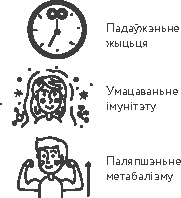
\includegraphics[scale=1.5]{willpower/ch5/4.pdf}
\end{figure}

Таўсьцейшыя людзі сядзяць на дзьве гадзіны даўжэй, чым людзі са звычайнай масай цела. Узьнікае заганнае кола: чым больш сядзім, тым таўсьцейшымі робімся, а~чым таўсьцейшымі мы робімся, тым цяжэй нам рухацца. Як апэтыт прыходзіць падчас ежы, так і цяглічная радасьць зьяўляецца пасьля руху. Чым актыўней мы рухаемся, тым лягчэй нам гэта рабіць, тым лепей працуюць цягліцы і тым болей задавальненьня мы атрымліваем і меней сядзім.

\subsection*{Тромбаўтварэньне}

Нерухомасьць зьвязаная з~павелічэньнем рызыкі тромбаў: чым менш працуюць ногі, тым мацнейшы застой, бо праца цягліцаў ніжніх канцавінаў важная для забесьпячэньня вэнознага звароту (т.зв. «цяглічнае сэрца»). Часьцей за ўсё тромбы ўтвараюцца ў~нагах, але могуць трапляць у~лёгкія (ТЭЛА~--- тромбаэмбалія лёгачнай артэрыі, у~25\,\% пры буйным тромбе надыходзіць раптоўная сьмерць), сэрца (інфаркт), мозг (інсульт), выклікаючы цяжкія наступствы. Пастаянная ўмераная побытавая фізычная актыўнасьць~--- важны чыньнік даўгалецьця, у~тым ліку для прафіляктыкі тромбаўтварэньня.

Навукоўцы апісваюць «офісны трамбоз», «трамбоз вандроўцы», «трамбоз геймэра»: апісаныя неаднаразовыя выпадкі, калі геймэры атрымлівалі гострыя трамбозы ног пры працяглай гульні і паміралі ад ТЭЛА. Спалучэньне нерухомасьці, абязводжваньня і стрэсу (адрэналін узмацняе зьвінаньне крыві) правакуе гэтыя выпадкі. Іншыя прычыны нерухомасьці: пералёты, падарожжы, шпіталізацыі, сядзячая праца. Кожныя дзьве гадзіны за кампутарам звыш мяжы ў~2,5 гадзіны павышаюць рызыку трамбозу лёгачнай артэрыі на 40\,\%.

\textbf{Эвалюцыйна нам патрэбныя розныя спосабы актыўнасьці.} Мы, як нашчадкі паляўнічых-зьбіральнікаў, маем патрэбу ў~працяглай нізкаінтэнсіўнай нагрузцы~--- як зьбіральнікі, і ў~сярэдняй або высокаінтэнсіўнай~--- як паляўнічыя і ваяры. Паляваньне~--- гэта працяглая хада, затым бег (перасьлед здабычы), у~пэўны момант часу набор высокай хуткасьці й магутнасьці.

\infobox{Ідэальнага і прыдатнага для ўсіх спорту няма, але ёсьць камбінацыя розных відаў актыўнасьці, аптымальная для большасьці людзей.}

Гэтая структура фізычнае актыўнасьці можа быць уяўленая ў~выглядзе пірага. Разумею, што мэтафара пірага як мадэлі рухомасьці ня вельмі здорава гучыць, затое навочна дэманструе, як усё працуе. Такім чынам, цеста пірага~--- гэта нетрэніроўная актыўнасьць, а~вось начыньне~--- адмысловыя заняткі спортам або любая іншая фізычная нагрузка. Таму спачатку трэба «замясіць цеста», то бок стварыць дастатковы і пастаянны ўзровень нетрэніроўнай актыўнасьці, а~затым дадаваць «начыньне».

Таксама фізычную актыўнасьць можна паказаць у~выглядзе піраміды, дзе на вяршыні знаходзяцца высокаінтэнсіўныя трэніроўкі, а~ўнізе~--- нізкаінтэнсіўныя.

\textbf{Мэта:}
\begin{itemize}
  \item высокаінтэнсіўная фізычная актыўнасьць: мінімум 4--6 хвілінаў на дзень, оптымум~--- 10 хвілінаў, ня больш за 3 трэніроўкі на тыдзень; 
  \item сярэднеінтэнсіўная аэробная фізычная актыўнасьць: каля 3--4 гадзінаў на тыдзень;
  \item шмат нетрэніроўнай актыўнасьці: ня менш за 7--10 тысячаў крокаў ці 4--6 гадзінаў «ня седзячы».
\end{itemize}

Такое спалучэньне сілавых і аэробных трэніровак, дастатковы час хадзьбы і скарачэньне часу сядзеньня на крэсьле працуе лепш за ўсё. Дасьледаваньні паказалі, што злучэньне некалькіх тыпаў мацней паляпшае фізычную працаздольнасьць, чым даўжэйшыя заняткі адным відам спорту.

\subsection*{Пытаньні і заданьні}

1. Як мяняецца ваша самаадчуваньне, калі вы рухаецеся шмат? А калі седзіце ўвесь дзень?

2. Ці заўважалі вы, што былыя спартоўцы пасьпяховыя і ў~бізнэсе?

3. Ці зьвярталі вы ўвагу, што нават пры захворваньнях умераная фізычная актыўнасьць паляпшае стан?


\section{Меней сядзець}

Часта на кансультацыях людзі скардзяцца, што ў~іх літаральна няма сілаў рухацца, яны хутка стамляюцца, адчуваюць сябе дрэнна, а~рух узмацняе апэтыт. Няўжо трэба сябе ламаць і прымушаць бегаць, калі ня хочацца? А рэч у~тым, што пры атлусьценьні, а~таксама пры шэрагу іншых станаў, такіх як лептынарэзыстэнтнасьць ды інсулінарэзістэнтнасьць, пры выгараньні, дэпрэсіі, арганізм як бы пераходзіць у~«энэргазьберагальны рэжым», павялічваючы спажываньне калёрыяў і зьніжаючы актыўнасьць. Таму пачынаць у~такім разе трэба з~простай актыўнасьці, з~рухаў, якія прыносяць задавальненьне.

Давайце разьбяромся, што мы павінны прыбраць са свайго жыцьця для паляпшэньня фізычнае актыўнасьці. 

\infobox{Самае важнае~--- гэта скараціць агульны час, праведзены седзячы і лежачы, і разьбіць прамежкі доўгага становішча седзячы на драбнейшыя, зрабіўшы рухальную актыўнасьць раўнамернай на працягу дня.}

\textbf{Меней сядзець.} Становішча седзячы~--- гэта асноўная форма гіпадынаміі, на другім месцы~--- становішча лежачы. Больш за палову ўсіх людзей праводзяць свой дзень, седзячы ў~самых розных формах: у~офісе, за стырном аўтамабіля, дома ў~фатэлі і да т.~п. Калі мы сядзім, то цягліцы кора (восевыя цягліцы цела, якія ўдзельнічаюць у~падтрыманьні цела) не працуюць, таму ў~становішчы седзячы і лежачы мы трацім менш калёрыяў, сэрцу цяжэй прапампоўваць кроў, плюс назапашваецца яшчэ цэлы набор нэгатыўных наступстваў.

\textbf{Сядзеньне звыш 4--6 гадзінаў на дзень наносіць нам шкоду, якая толькі часткова кампэнсуецца фізычнымі практыкаваньнямі.} У выніку працяглага сядзеньня ў~цягліцах на 90\,\% памяншаецца актыўнасьць фэрмэнту ліпапратэінліпазы, якая расшчапляе тлушчы. Кароткая і сярэдняя працягласьць нагрузкі істотна не ўплывае на гэты працэс. Галоўная задача~--- скарачаць час, праведзены ў~становішчы седзячы: падлічыць, колькі гадзінаў на дзень вы седзіце, жахнуцца гэтаму і скласьці плян па скарачэньні гэтага часу.

\subsection*{Што рабіць? Першая ідэя~--- устаць}

Нашы продкі садзіліся толькі для адпачынку, калі стамляліся. Многія доўгажыхары, хоць і не займаюцца спэцыяльна спортам, цэлы дзень знаходзяцца ў~руху і амаль не сядзяць. Карысна частку сядзячай працы перанесьці ``на ногі'' і пачаць працаваць стоячы. У гэтым няма нічога незвычайнага: яшчэ нядаўна людзі працавалі стоячы, за канторкамі. Калі мы працуем стоячы, у~нас задзейнічаныя буйныя групы цягліц, а~нагрузка на сьпіну ў~два разы меншая ў~параўнаньні зь сядзеньнем.

\begin{figure}[htb!]
  \centering
  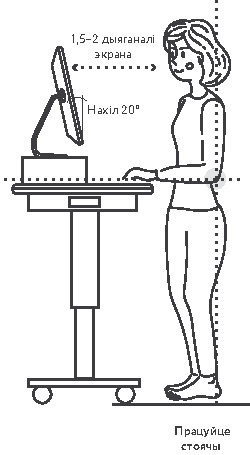
\includegraphics[scale=1.5]{willpower/ch5/5.pdf}
\end{figure}

\emph{Цяпер існуе вялікая колькасьць сталоў і спэцыяльных падставак для працы стоячы~--- вы можаце выбраць на свой густ. Галоўнае~--- сачыце за базавай эрганомікай.}

Праца стоячы спальвае на 1,36 кілакалёрыяў у~хвіліну больш, чым сядзеньне. Гэта амаль 80 дадатковых калёрыяў у~гадзіну. Стаяньне на працягу дзьвюх гадзінаў на 2\,\% зьніжае ўзровень глюкозы ў~крыві і на 11\,\%~--- узровень трыгліцерыдаў. Становішча стоячы~--- гэта больш моцная поза, таму мы лепей трываем стрэс і падвышаем прадуктыўнасьць, бо пракрастынаваць стоячы нашмат складаней.

\subsection*{Скарачайце колькасьць гадзінаў, праведзеных седзячы, і дома}

Прагляд тэлевізара, кампутарныя гульні і да т.~п. таксама шкодныя. Любімы сэрыял можна паглядзець і зь велатрэнажора, а~ад тэлевізара варта наогул адмовіцца: глядзець «скрыню»~--- гэта ўжо мавэтон.

\emph{Сядзеньне сядзеньню ня роўнае. Назіраючы за сваімі дзецьмі, я заўважаю, што яны актыўна выкарыстоўваюць позу на кукішках, паднімаючы рэчы з~зямлі і разглядаючы казюрак. У эўрапейскай культуры існуе негалоснае табу на сядзеньне на кукішках, лічыцца, што так сядзяць некультурныя ці чужыя людзі. Аднак са старажытных часоў, дзясяткі тысячаў гадоў таму назад, людзі часта сядзелі на кукішках. Рэч у~тым, што пры сталым выкарыстаньні гэтай позы на касьцях утворацца дадатковыя паверхні~--- фасэткі. Таму тым людзям, хто не сядзіць так зь дзяцінства, поза здаецца нязручнай як праз асаблівасьці разьвіцьця шкілета, так і праз скарочанае ахілесава сухажыльле. Напрыклад, у~Японіі больш за 20\,\% маладых людзей ужо ня могуць пратрымацца некалькі хвілінаў у~гэтай позе.}

\emph{Навукоўцы, дасьледуючы лад жыцьця паляўнічых-зьбі\-раль\-ні\-каў хадза, выявілі, што яны даволі шмат сядзяць. Вывучэньне паказала, што з~пункту гледжаньня біямэханікі сядзеньне на кукішках дае нашмат больш высокую статычную нагрузку на цягліцы ног і кора, чым звычайнае сядзеньне, набліжаючыся да хады! Гэта вядзе і да меншых рызыкаў для здароўя. Поза на кукішках можа быць адным з~элемэнтаў дынамічнае позы, разам зь сядзеньнем на крэсьле, з~працай стоячы, працай лежачы. Акрамя таго, так бясьпечней за ўсё паднімаць нешта з~падлогі і нашмат карысьней для здароўя зьдзяйсьняць у~ёй дэфэкацыю. На жаль, некаторым будзе складана яе выкарыстаць з~ужо апісаных анатамічных прычынаў.}

\subsection*{Выкарыстоўвайце дынамічную позу}

Зьмена позы дапамагае пазьбегнуць зацяканьня цягліцаў, падвысіць прадуктыўнасьць. Ня трэба стаяць гадзінамі: як толькі адчулі стому ў~нагах~--- сядайце і працуйце седзячы. Доўгае нерухомае стаяньне таксама можа нашкодзіць. Для адпачынку на 15 хвілінаў закіньце ногі на стол або сьцяну вышэй за ўзровень галавы~--- гэта паляпшае адток крыві. Вы можаце прыдумаць любыя зручныя вам працоўныя позы~--- галоўнае не захрасаць у~іх надоўга. Працуйце пэрыядычна лежачы~--- гэта падвышае крэатыўнасьць.

\begin{figure*}[htb!]
  \centering
  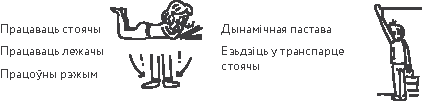
\includegraphics[scale=1.5]{willpower/ch5/6.pdf}
\end{figure*}

\emph{Поза напаўлежачы не перагружае хрыбет і падабаецца многім. Напрыклад, Максім Багдановіч звычайна чытаў і пісаў толькі лежачы, лежачы працавалі палітык Уінстан Чэрчыль, пісьменьнік Марк Твен, а~філёзаф Томас Гобс неяк нават пасьпісваў усе прасьціны~--- настолькі яму не хацелася вылазіць з-пад коўдры па паперу.}

\infobox{Становішча стоячы~--- гэта «мацнейшая» поза, таму мы лепш пераносім стрэс і павялічваем прадукцыйнасць, бо пракрастынаваць стоячы заўважна складаней!}

\subsection*{Рабіце перапынкі}

Небясьпечны ня толькі агульны час сядзеньня, але й працяглыя эпізоды нерухомасьці. Навукоўцы давялі, што чым больш перапынкаў, тым карысьней для здароўя: гэта ўплывае на аб'ём таліі, масу цела, узровень глюкозы і тлушчаў у~крыві. Таму старайцеся рабіць перапынкі, кожную гадзіну ўстаючы з-за стала хаця б на хвіліну. Нават калі вы прыўстанеце ўсяго на некалькі сэкундаў і проста сядзеце па-іншаму чыста анатамічна, будзе менш зацяканьня ў~целе і лепш для вас.

\subsection*{Запоўніце перапынкі рухам}

Нават дзьве хвіліны фізычнай актыўнасьці могуць аказаць істотны ўплыў на здароўе. Такія перапынкі карысныя і для прадуктыўнасьці, бо перадухіляюць стомленасьць і выгараньне. Купіце пясочны гадзіньнік на 2--3-5 хвілін для міні-перапынкаў. Схадзіце да калегаў, падыдзіце да акна, спусьціцеся па лесьвіцы, выйдзіце на вуліцу і назад, выпіце вады, а~калі ваш «сядзячы мозг» будзе спакушаць вас вольным месцам у~транспарце~--- не паддавайцеся яму!

\emph{\textbf{Поза пры апаражненьні.} Седзячы на звычайным унітазе, вы разьмяшчаеце кішачнік пад нефізыялягічным вуглом, абезрухамляеце пубарэктальные цягліцы, якія патрэбныя для ўдзелу ў~працэсе. Поза прыкметна ўплывае на працэс дэфэкацыі, які ўключае ступень ціску, паўнату апаражненьня і яго лёгкасьць.}

\emph{Нездаровы анарэктальны вугал павышае ціск у~кішачніку і ўнутрыбрушны ціск (рызыка кілаў!), што зьяўляецца чыньнікам рызыкі разьвіцьця шэрагу хваробаў, ад запораў і гемарою да сындрому раздражнёнага кішачніка. Падвышаны ціск можа нават спрыяць парушэньню працы ілеацэкальнай засланкі і закіду зьмесьціва тоўстага кішачніка ў~тонкі.}

\emph{Ужо шмат гадоў у~мяне стаіць падстаўка пад унітазам, вядомая як Squatty Potty, навуковая назва~--- прылада для пастуральнай мадыфікацыі дэфэкацыі (defecation postural modification devices or DPMDs). Дасьледаваньні паказваюць, што выкарыстаньне такіх падставак дапамагае ня толькі людзям з~запорамі, але паляпшае дэфэкацыю і ў~здаровых людзей, дапамагае пры праблемах з~мочаспусканьнем у~жанчынаў, у~т.л. і пры цяжарнасьці, пры сындроме раздражнёнага кішачніка, гемароі. Вядома, падстаўка ня вырашыць усіх праблемаў з~запорамі, але дапаможа прыкметна зьменшыць рызыкі ад нефізіялягічнага сядзеньня.}

\subsection*{Пытаньні і заданьні}

1. Колькі гадзінаў на дзень вы седзіце?

2. Як вы можаце дадаць працу стоячы ў~свой графік? Складзіце сьпіс: не садзіцца ў~транспарце, размаўляць стоячы, частку працы рабіць стоячы, чытаць стоячы і да т.~п.

3. Купіце спэцыяльны працоўны стол або ўсталюеце стойку для працы стоячы.


\section{Болей нетрэніроўнай актыўнасьці}

\begin{figure*}[htb!]
  \centering
  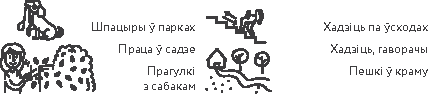
\includegraphics[scale=1.5]{willpower/ch5/7.pdf}
\end{figure*}

Нетрэніроўная актыўнасьць~--- гэта ўвесь аб'ём паўсядзённай актыўнасьці, уключаючы хатнія справы, працу, камунікацыю і інш. Аб'ём гэтай нагрузкі можа вар'іравацца ў~розных людзей ад 300 ккал да 800 ккал і нават больш. Да яе адносіцца, напрыклад, хадзьба пешшу, пад'ём па лесьвіцы, паход у~краму, работа ў~доме, у~садзе, актыўная гэстыкуляцыя.

\emph{Сярод доўгажыхароў у~самых розных пунктах зямлі няма спартоўцаў, якія бегаюць маратоны або падымаюць вялізныя цяжкасьці. Вось, напрыклад, пастухі ў~Сардзініі~--- у~іх шмат нізкаінтэнсіўнай фізычнай актыўнасьці, як і ў~нашых продкаў паляўнічых-зьбіральнікаў.}

\textbf{Дасьледаваньні паказваюць, што з~2008 па 2013 год мы пачалі хадзіць на 800--1500 крокаў менш!}

\textbf{Самы просты спосаб павялічыць нетрэніроўную актыўнасьць~--- пачаць больш хадзіць.} Хадзьба ня толькі карысная для фізычнага здароўя, але й паляпшае настрой, зьніжае гнеў, трывожнасьць і стомленасьць, яна больш аздараўленчая, чым, напрыклад, расьцяжка. Гэта тое, што лёгка паддаецца кантролю з~дапамогай тэлефона, і тое, што вы можаце зрабіць проста зараз.

\textbf{Хадзьба}~--- гэта базавы і просты спосаб, і нагрузку можна вымераць з~дапамогай крокамера. Крытэрыі могуць быць любымі~--- каму гадзіна хадзьбы, каму 7--12 тысячаў крокаў штодня. Навукоўцы лічаць, што 7500 крокаў~--- гэта мінімальны паказьнік, які абараняе вашае здароўе, а~вось 12 500~--- аптымальны! Прайдзіце ўсяго 15 хвілінаў пасьля прыёму ежы~--- гэта дазволіць зьнізіць уздым ўзроўню глюкозы ў~крыві. 

\emph{Тыя, хто не трэніраваўся, але працаваў па гаспадарцы ці больш хадзіў, маюць на 27\,\% ніжэйшую рызыку інфаркту і на 30\,\% ніжэйшую за рызыку сьмерці ў~параўнаньні з~тымі, у~каго няма і такой актыўнасьці.}

Старайцеся, каб хадзьба не патрабавала асобных затратаў часу, а~была ўкаранёная ў~структуру вашага жыцьця. Напрыклад, хадзіце размаўляць з~калегамі, абмяркоўвайце справы ідучы, паркуйцеся крыху далей ад дома, сустракайцеся ў~парку, завядзіце сабаку, слухайце аўдыякніжкі на хаду, адпраўляйцеся ў~больш далёкую краму і да т.~п. Каб выступленьні калегаў былі карацейшыя, скарыстайцеся старажытнай парадай~--- выступайце, стоячы толькі на адной назе. І самі трэніруйце балянс у~хатніх умовах: чысьціце зубы, стоячы па чарзе то на адной, то на другой назе.

\textbf{Можна зрабіць хадзьбу яшчэ больш эфэктыўнай:} датрымлівайцеся пэўнага пульсу, паскарайцеся пэрыядычна, выбірайце няроўную паверхню (пясок, зямля ў~парку), паднімайцеся па лесьвіцах~--- гэта спальвае нават больш калёрыяў, чым бег. Хадзьба на лыжах і скандынаўская хада пераўзыходзяць звычайную: магчыма, вы знойдзеце групу аматараў «пахадзіць з~палкамі» у~вашым раёне~--- цяпер гэта вельмі папулярны від спорту.

Варта арганізаваць сваё жыцьцё так, каб хадзіць болей: напрыклад, жыць у~прыватнай хаце, каб была магчымасьць гуляць на прыродзе і займацца садам. Завесьці сабаку~--- так, уладальнікі сабак ня толькі праходзяць на 2800 крокаў больш, але і нашмат лепш захоўваюць свой рэжым дня, часьцей бываюць на сонцы, адчуваюць менш стрэсу, радзей пакутуюць на атлусьценьне.

\textbf{Дарога на працу.} Дасьледаваньні паказваюць, што занадта доўгая дарога на працу, заторы зьяўляюцца сур'ёзнымі пагрозамі для здароўя. Чым даўжэй вы едзеце на працу, тым вышэйшая рызыка атлусьценьня і мэтабалічных парушэньняў (глюкоза, ліпідны профіль і да т.~п.). Гараджане, якія ходзяць на працу пешшу і жывуць каля працы, маюць і больш здаровую масу цела. Працягласьць дарогі на працу звыш 30 міляў зьвязаная з~павелічэньнем сьмяротнасьці. Заторы~--- гэта бізун нашага часу. Напрыклад, толькі Лондан Сіці штодня губляе за кошт затораў мільён фунтаў, а~агульныя выдаткі часу, паліва і да т.~п. складаюць у~ЗША больш за сотню мільярдаў даляраў за год. Мы так ня любім заторы, ажно гатовыя ахвяраваць 5 хвілінамі вольнага часу, каб на хвіліну менш стаяць у~заторы. Не сядзіце ў~грамадскім транспарце, па магчымасьці дабірайцеся на працу актыўна, пешшу або на ровары, паркуйцеся ці выходзьце з~мэтро трошкі раней, каб прайсьці крыху пешшу.

\subsection*{Пытаньні і заданьні}

1. Колькі крокаў за дзень вы праходзіце? Палічыце з~дапамогай смартфона. Паспрабуйце розныя віды хадзьбы.

2. Як вы можаце дадаць хадзьбу ці іншую актыўнасьць у~свой працоўны дзень?

3. Знайдзіце прыгожыя і зручныя маршруты для працяглых пешых шпацыраў.


\section{Аэробная актыўнасьць}

Чаму бег з~раніцы так уздымае настрой? Бо нічога горшага з~вамі на працягу дня ўжо ня здарыцца! А калі бяз жартаў, то ўцячы ад шматлікіх праблемаў са здароўем сапраўды можна, калі вы дадасьце больш аэробнай актыўнасьці. Гэта практыкаваньні лёгкай ці сярэдняй інтэнсіўнасьці, сярод якіх~--- бег, ровар, танцы, фітнэс, канькі, скачкі са скакалкай і да т.~п. Важна адзначыць, што такія віды трэніровак здольныя павярнуць назад атэрасклероз і рэальна палепшыць стан вашага сэрца і артэрый, «амаладзіць» іх.

\emph{Згодна зь некаторымі дасьледаваньнямі, практыкаваньні на трывушчасьць і інтэрвальныя трэніроўкі лепш запавольваюць старэньне, чым узьняцьце цяжараў. Тыя дарослыя, якія бегаюць па паўгадзіны пяць разоў на тыдзень, маюць тэламэры, якія адпавядаюць узросту на 10 гадоў маладзейшаму.}

\textbf{Калі вы толькі пачынаеце свае кардыё-трэніроўкі, пажадана карыстацца пульсамерам.} \emph{Разьлічыце свой максімальны пульс (220 -- узрост) і ад яго вылучыце наступныя зоны:}
\begin{itemize}
  \item \emph{разьмінкі~--- 50--60\,\% ад максімальнага;}
  \item \emph{аднаўленьні~--- 60--70\,\%;}
  \item \emph{фітнэс~--- 70--80\,\%;}
  \item \emph{аэробная~--- 80--90\,\%;}
  \item \emph{анаэробная~--- 90--95\,\%;}
  \item \emph{максімальная нагрузка~--- больш за 95\,\% ад максімальнага пульсу.}
\end{itemize}

Аптымальна большую частку часу праводзіць у~фітнэс-зоне, не пераходзячы ў~анаэробную і максімальную. Вядома, гэты падзел даволі ўмоўны і шмат хто ўжо лічыць яго састарэлым, бо тлушч спальваецца пры любой нагрузцы. Умоўна кажучы, аэробны рэжым~--- гэта калі вы ня можаце спакойна размаўляць падчас нагрузкі.

Яшчэ прасьцейшая формула: аэробная актыўнасьць у~шырэйшым дыяпазоне ЧСС~--- ад 65\,\% да 80\,\% ад максімальнага пульсу (220~--- узрост).

\textbf{Зь біяхімічнага пункту гледжаньня вылучаюць:}
\begin{itemize}
  \item аднаўленчы (кампэнсаторны) рэжым, калі ўзровень прадукту акісьленьня глюкозы лактату ніжэйшы за 2 ммоль / л, то бок такая хуткасьць бегу, калі вы можаце размаўляць, не адчуваючы прыкметных цяжкасьцяў у~дыханьні;
  \item аэробная зона~--- паміж аэробным і лактатным парогам (узровень лактату вышэйшы за 4 ммоль / л), калі вы можаце пры бегу рабіць на 4 крокі ўдых і на 4 крокі выдых;
  \item анаэробная зона, калі лактат расьце яшчэ вышэй, і дыхаць можна толькі 3 крокі ўдых~--- 3 крокі выдых. Для трэніровак аптымальна прытрымлівацца аэробнай зоны.
\end{itemize}

\infobox{Простая і карысная фізычная актыўнасьць~--- гэта павольны бег трушком працягласьцю да 45 хвілін, з~пульсам 60--80\,\% ад максімальнага сумарна ад 150 да 360 хвілінаў на тыдзень, г.~зн. ад 3 да 5 трэніровак.}

Для бегу выбірайце прыгожае месца са сьвежым паветрам, зручны абутак, азнаёмцеся зь біямэханікай бегу і стартуйце. Перавагі аэробнай актыўнасьці ў~тым, што яна бадзёрыць, уцягвае, дае цяглічную радасьць, мае мала пабочных эфэктаў, не патрабуе глыбокага засваеньня тэхнікі, плюс яе можна рабіць у~групе ці з~партнёрам.

\subsection*{Тэхніка бясьпекі пры бегу}

Прызямляцца варта на мысок роўна пад цэнтрам цяжару цела. Імкніцеся не рабіць занадта доўгія крокі, няхай будзе для пачатку каля 90 крокаў у~хвіліну. Рукі ў~ідэале павінны быць сагнутыя і рухацца ўздоўж цела. Калі вы пачынаеце бегчы, ня горбіцеся, трымайце калені мяккімі, глядзіце наперад, а~не ў~зямлю. Удыхайце паветра носам, дыхайце раўнамерна. У працэсе бегу не разгойдвайцеся, сярэдняя лінія вашага цела павінна быць стабілізаваная. Перад трэніроўкай абавязкова рабіце разьмінку, прынамсі 10 хвілінаў лёгкага бегу ці хуткай хадзьбы.

Пачынайце з~20-хвілінных прабежак 2--4 разы на тыдзень, цалкам нармальна першы час пэрыядычна пераходзіць на крок. Навічкі могуць чаргаваць хвіліну бегу і хвіліну хуткай хадзьбы і рабіць так па 10--15 разоў. 2--3 такія трэніроўкі на тыдзень будзе цалкам дастаткова, празь некалькі месяцаў можна дадаць дадатковую трэніроўку. Абавязкова сьпіце даўжэй, каб лепш аднаўляцца.

\begin{figure}[htb!]
  \centering
  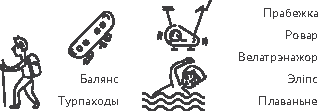
\includegraphics[scale=1.5]{willpower/ch5/8.pdf}\\
  \medskip
  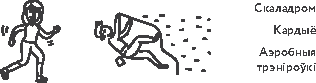
\includegraphics[scale=1.5]{willpower/ch5/9.pdf}
\end{figure}

Ваш натуральны тэмп павінен даваць магчымасьць казаць поўнымі сказамі: калі размаўляць цяжка, вы перавышаеце сваю аптымальную хуткасьць. Хуткае павышэньне нагрузкі прыводзіць да траўмаў, таму не павялічвайце штотыдзень колькасьць кілямэтраў больш, чым на 10\,\%. Важнае і пачуцьцё меры, бо залішні аб'ём трэніровак падвышае рызыку траўмаў: калена бегуна, запаленьне ахілесава сухажыльля, сындром расколатай галёнкі і інш. Бегайце ў~адмысловым бегавым абутку. Ідэальна бегаць па грунце, яшчэ лепш~--- па перасечанай мясцовасьці з~прыгожымі краявідамі.

\subsection*{Дадайце няўстойлівасьці}

Невідавочная пагроза для нашых цягліцаў~--- гэта роўныя паверхні. Роўная падлога, дарожка, калідор… гучыць і выглядае выдатна, дзе ж праблема? Рэч у~тым, што наша рухальная сыстэма эвалюцыйна прыстасаваная да руху па няроўных паверхнях. Сыстэмы раўнавагі і каардынацыі без належнай нагрузкі заўчасна атрафуюцца, мы страчваем плястычнасьць і ўстойлівасьць. З узростам гэта прыводзіць да ўзмацненьня крохкасьці і прыкметнага зьніжэньня якасьці жыцьця.

\emph{Навукова ўстаноўлена, што хадзьба, бег і трэніроўкі на пяску заўважна адрозьніваюцца ад аналагічных на траве або на цьвёрдай паверхні. Пры занятках на пяску зьмяншаецца рызыка траўмаў, узмацняецца расход энэргіі пры выкананьні аднолькавага аб'ёму практыкаваньняў, павялічваецца адаптацыя, лепш трэніруецца раўнавага, павялічваецца максімальнае спажываньне кіслароду.}

\textbf{Дадайце больш няўстойлівасьці ў~сваё жыцьцё і трэніроўкі.} Ёсьць мноства прыстасаваньняў: балянсіры, батуты, фітдыскі, нацяжныя канаты і інш. Чым менш вакол нас пастуральных, то-бок зьвязаных з~утрыманьнем паставы выклікаў, тым горшыя наша пастава і цяглічная сыстэма. Таму элемэнты няўстойлівасьці~--- як у~трэніроўках, так і ў~жыцьці~--- гэта проста, весела і вельмі карысна.

\subsection*{Трэйлранінг}

\textbf{Трэйлранінг} (trail running), альбо бег па мяккіх паверхнях, уцягвае ў~работу і ўмацоўвае больш цягліцаў ног і корпуса, чым бег па асфальце, а~таксама зьмяншае нагрузку на зьвязкі і косткі. Бег па прамой цыклічны, а~бег па прыродным маршруце не ўтрымлівае аднолькавых участкаў. Калі мы манатонна бяжым па асфальце, кожны крок падобны на папярэдні, і мы прызямляемся ступаком абсалютна аднолькава, гэта выклікае перагрузку і павялічвае рызыку траўмы. Пры бегу на прыродзе мы ставім нагу кожны раз крыху па-іншаму, і гэта раўнамерней разьмяркоўвае ўдарную нагрузку: даведзена, што бег па траве зьмяншае нагрузку на ступні на 17\,\% у~параўнаньні зь бегам па асфальце. Апроч фізычнае карысьці, такі бег патрабуе нашмат больш увагі, цалкам паглынае ваш розум, падтрымлівае засяроджанасьць. Так, трэба ўвесь час зьмяняць даўжыню кроку, пралічваць рухі на 5--6 крокаў наперад~--- і гэта дазваляе выдатна перазагружацца. Акрамя таго, больш разнастайнасьці і візуальнага задавальненьня заўсёды карысна для настрою і для здароўя.

\subsection*{Пытаньні і заданьні}

1. Ці любіце вы бегаць?

2. Што можа матываваць вас да прабежкі? Модная форма і красоўкі? Прыгожы краявід? Партнёр па прабежцы? А калі ўсё адразу?

3. Ці маеце ровар? Ці часта вы ім карыстаецеся?


\section{Анаэробная актыўнасьць}

У мяне ў~габінэце вісіць турнік, а~пад ім ляжаць гантэлі і гіра. Гэта ня арт-інсталяцыя, а~крыніца бадзёрасьці падчас працоўнага дня. За некалькі хвілінаў я магу ня толькі нагрузіць свае цягліцы, але й палепшыць разумовыя здольнасьці і ўзбадзёрыцца, не зьвяртаючыся да кафэіну.

Анаэробная актыўнасьць~--- гэта практыкаваньні, для выкананьня якіх энэргія выпрацоўваецца пры акісьленьні глюкозы ў~адсутнасьці кіслароду. Калі аэробная актыўнасьць уключае больш-менш раўнамерныя практыкаваньні, то анаэробныя трэніроўкі звычайна маюць выразную пэрыядызацыю: спачатку актыўная праца, затым адпачынак, па прынцыпе «трэніруйся каротка, але цяжка». Да іх адносяцца сілавы спорт, армрэсьлінг, красфіт, спрынт і да т.~п. Многія віды актыўнасьці могуць быць выкананыя ў~розных рэжымах: бег-спрынт і бег трушком, спрынт на ровары і спакойная велапрагулка.

\subsection*{Разнастайце бег}

Спачатку 100 мэтраў спрынту, потым 300 мэтраў пешшу, аднавіць дыханьне, затым зноў спрынт на максімальнай хуткасьці. Але такі від трэніроўкі не пасуе пачаткоўцам і супрацьпаказаны пры некаторых захворваньнях. Замест таго каб выконваць нагрузку «да канца», карысьней трэніравацца пры 80--90\,\% пульсу ад максімальнага. Такая актыўнасьць павялічвае ўзровень тэстастэрону, спрыяе цяглічнаму росту, дабратворна адбіваецца на здароўі костак і яшчэ на мностве іншых паказьнікаў арганізма.

\subsection*{Базавыя практыкаваньні}

Сярод размаітасьці ўсемагчымых практыкаваньняў перавагу трэба аддаць базавым~--- не ізаляваным,~--- якія залучаюць вялікую колькасьць цяглічных груп і выконваюцца са свабоднымі вагамі або вагой свайго цела. Гэта палеатрыяда «штурхай-цягні-брыкай». 

\textbf{Штурхальныя рухі} (адштурхваем ад сябе) уключаюць удары, кідкі, кіданьне прадметаў, адцісканьні і жымы. 

\textbf{Цягальныя рухі} (прыцягваем сябе ці да сябе) уключаюць узьняцьце цяжараў, лазаньне па канаце, скалалазаньне, падцягваньні і цягі. 

\textbf{Брыкальныя рухі} (адштурхваем/адштурхваемся нагамі) уключаюць скачкі, прысяданьні, выпады, удары нагамі. 

\textbf{Практыкаваньні з~вольнымі вагамі} працуюць лепш за ўсё, бо яны маюць поўны кінэтычны ланцуг, дзе перадача высілкаў ідзе ад падлогі да рук праз усё цела. Таксама практыкаваньні дапамагаюць утрымліваць раўнавагу і лепш прыкладаць сілу. Для хатніх умоў выдатна пасавацьмуць гіры~--- гэта зручна і эфэктыўна пры датрыманьні тэхнікі практыкаваньняў.

\textbf{Сілавыя практыкаваньні.} У прафэсійным спорце гэта жым лежачы, станавая цяга, прысяданьні са штангай. У хатніх умовах вы можаце рабіць прысяданьні, падцягваньні на турніку і адцісканьні, працуючы са сваёй вагой. Выпады, адцісканьні на брусах, заскакваньні, жым над галавой, практыкаваньні з~гірай, жым штангі стоячы, бэрпі~--- гэта прыклады іншых відаў базавых практыкаваньняў, якія даюць найлепшы эфэкт для росту цягліцаў. Навічкі могуць цалкам скласьці зь іх сваю трэніроўку. 

\infobox{Базавыя практыкаваньні патрабуюць ідэальнай тэхнікі, бо іх няправільнае выкананьне зь вялікімі вагамі павялічвае рызыку траўмы нават пры невялікіх памылках.}

У кожным практыкаваньні спачатку вызначыце сваю максімальную вагу (досьледным шляхам і з~дасьведчаным трэнерам!), а~трэніруйцеся з~вагамі 60--75\,\% ад максімуму~--- такая нагрузка добра пасуе для актывацыі росту розных цяглічных валокнаў. Сярэдні дыяпазон паўтораў (8--12 разоў) аптымальны для максімальнага росту цягліцаў, нізкая колькасьць паўтораў (1--5 разоў) зь яшчэ большымі вагамі паляпшае нэрвова-цяглічную адаптацыю.

Навічкам, людзям 40+ і ўсім, хто не імкнецца да рэкордаў, лепш выконваць практыкаваньні зь нізкай інтэнсіўнасьцю і максімальнай колькасьцю паўтораў~--- гэта карысьней для росту цягліцаў і аптымальна для даўгалецьця. Рэкамэндуецца выконваць практыкаваньні з~30--60\,\% максімальнай вагі і дыяпазонам паўтораў 15--20 разоў. Калі трэніровачны аб'ём аднолькавы, то як высока-, так і нізкаінтэнсіўныя сілавыя практыкаваньні даюць падобныя вынікі. Варта заўважыць, што \textbf{рызыка ўскладненьняў пры сярэднеінтэнсіўных сілавых трэніроўках яшчэ меншая, чым пры кардыянагрузках.}

\begin{figure}[htb!]
  \centering
  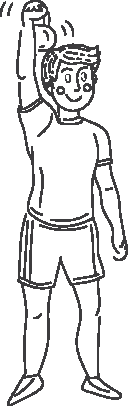
\includegraphics[scale=1.5]{willpower/ch5/10.pdf}
\end{figure}

Пры рэгулярным выкананьні нават адна трэніроўка на тыдзень дае рост цягліцаў, аптымальна дзьве-тры трэніроўкі на тыдзень, але ня больш~--- важна пазьбягаць ператрэніраванасьці. Зьніжэньне сілавых вынікаў, страта задавальненьня ад трэніроўкі, млявасьць~--- сымптомы перагрузкі. Трэніруйцеся рэдка, але інтэнсіўна.

\emph{Павялічыць нагрузку можна, напрыклад, зьмяніўшы хуткасьць уздыму цяжараў, робячы вельмі павольную сілавую трэніроўку. Пры ёй цягліцы нашмат даўжэй знаходзяцца пад нагрузкай, што выклікае вялікую стомленасьць і зьяўляецца стымулам да цяглічнага росту.}

Аднатыпная праграма трэніроўкі, асабліва хатняй, стамляе. Вы можаце лёгка разнастаіць кожнае з~практыкаваньняў. Адціскацца можна, паставіўшы рукі на стосы кніг ці ногі~--- на ўзвышэньне, або нават на адной руцэ. А можна ўзяць гумовы джгут і адціскацца, заціснуўшы яго рукамі. Прысядаць можна дзясяткамі розных спосабаў, ад нажніцаў да прысяданьня на адной назе. Плянак існуе вялікая разнастайнасьць відаў~--- выбірайце і чаргуйце. Падтрымлівайце разнастайнасьць сваіх трэніровак, выбіраючы практыкаваньні, якія вам падабаюцца ці лепш пасую па біямэханіцы.

\subsection*{Пытаньні і заданьні}

1. Купіце дадому гантэлі і гіру з~магчымасьцю рэгуляваньня.

2. Ці ёсьць побач з~вамі пляцоўка з~турнікамі? Наведвайце яе~--- зможаце знайсьці аднадумцаў, што зробіць вашыя трэніроўкі больш займальнымі.

3. Для ўсіх практыкаваньняў з~вагой вывучыце тэхніку і засвойце яе пад кантролем трэнера.


\section{Высокаінтэнсіўныя інтэрвальныя практыкаваньні}

Часам у~спартовай залі я бачу, што людзі бавяць у~ім шмат часу, але марнуюць яго: сядзяць у~тэлефоне, глядзяць у~акно, безуважліва аглядаюць навакольных. Калі вы прыйшлі займацца, трэба быць максімальна сфакусаванымі і добра выкладвацца. Тады нават кароткая трэніроўка будзе карыснай і эфэктыўнай.

Сутнасьць сыстэмы высокаінтэнсіўнай інтэрвальнай трэніроўкі ВІІТ (HIIT) заключаецца ў~аб'яднаньні як аэробнага, так і анаэробнага падыходаў. Спачатку на кароткі прамежак (10--20 сэкундаў) часу мы перавышаем аэробны парог, выходзім у~анаэробную зону, затым вяртаемся назад, працуючы даўжэйшы пэрыяд зь нізкай нагрузкай. Гэта дазваляе нагружаць абодва тыпы цяглічных валокнаў, ствараць большы кіслародны голад, што стымулюе тлушчаспаленьне, таксама ВІІТ эфэктыўна павялічваюць адчувальнасьць да інсуліну. 

\infobox{Трэніроўкі ВІІТ досыць кароткія, 20--30 хвілінаў, падыходы адсочвайце з~дапамогай таймэра.}

Сярод розных сыстэмаў сваім мінімалізмам вылучаецца \textbf{табата}, дзе трэніроўка можа доўжыцца чатыры хвіліны і складаецца з~васьмі раундаў, дзе 20 сэкундаў займае выкананьне практыкаваньня, а~10 сэкундаў~--- адпачынак. Можна выканаць восем розных практыкаваньняў або чаргаваць меншую іх колькасьць. Падлічвайце колькасьць паўтораў у~кожным падыходзе і складайце іх~--- гэта дапаможа вам адсочваць прагрэс. Можна спампаваць табата-таймэры, каб было зручней прытрымлівацца раўндаў. Або тры наступныя сэрыі з~адпачынкам паміж імі па 3 хвіліны: 30 сэкундаў моцных практыкаваньняў, 15 сэкундаў адпачынку і так 8 разоў.

Таксама папулярны \textbf{красфіт}~--- камбінацыя элемэнтаў як ВІІТ, так і сілавых відаў спорту, бегу і да т.~п. У яго аснове ляжаць разнастайныя функцыянальныя рухі, якія выконваюцца з~высокай інтэнсіўнасьцю. Зрэшты, некаторыя дасьледнікі асьцерагаюцца, што шматлікія праграмы красфіту могуць быць небясьпечныя для здароўя.

\textbf{Прыклад практыкаваньняў}: 20-сэкундыя спрынты ў~спалучэньні з~60-сэкунднай хадзьбой ці бегам трушком. ВІІТ на велатрэнажоры: вы 30 сэкундаў круціце пэдалі, максімальна выкладваючыся, затым 60 сэкундаў~--- вельмі павольна, аднаўляючыся. У такім рэжыме можна рабіць бэрпі, бег ва ўпоры лежачы, заскокваньні на плятформу, практыкаваньні ``зорка'' (jumping jacks), ``скалалаз'', скачкі ``ўнутр-вонкі''.

\textbf{Нават 3--7--10 хвілінныя трэніроўкі карысныя.} Але каб яны працавалі, яны павінны быць высокаінтэнсіўнымі, інтэрвальнымі, задзейнічаць буйныя цягліцы ўсяго цела, уключаць сілавыя і аэробныя практыкаваньні. Выкарыстоўвайце шматсустаўныя базавыя практыкаваньні з~высокай энэргаёмістасьцю і не рабіце высокаінтэнсіўны раўнд даўжэй за 30 сэкундаў. 

\emph{Дасьледаваньне паказала, што нават невялікія ўсплёскі фізычнай актыўнасьці прыкметна ўплываюць на мэтабалізм. Паддосьледныя зь сядзячым ладам жыцьця круцілі пэдалі пяць разоў па 45 сэкундаў (160 сэкундаў сумарна за дзень) на працягу трох дзён. Пасьля прыёму ежы ўзровень тлушчаў у~крыві быў на 30\,\% ніжэйшы, чым да гэтага. Таму нават самая невялікая актыўнасьць лепшая, чым яе адсутнасьць. Адна хвіліна спрынту з~інтэрваламі ў~20 сэкундаў (тры разы па 20) тры разы на тыдзень на працягу трох месяцаў прыводзіла да паляпшэньня паказьнікаў сардэчна-сасудзістай сыстэмы і мэтабалізму.}

\subsection*{Пытаньні і заданьні}

1. Няма часу на трэніроўку? Знайдзіце чатыры хвіліны для табаты.

2. Паспрабуйце разнастаіць бег ці ровар, дадаючы ўдарныя адрэзкі паскарэньня.

3. Якія практыкаваньні з~вагой свайго цела вы ведаеце? Што яшчэ можаце да іх дадаць?


\section{Спантанная рухальная актыўнасьць}

Вядома, любая рухальная актыўнасьць і спорт карысныя для здароўя. Разнастайнасьць нашых рухаў можна ўмоўна падзяліць на адвольна-валявыя, якія выконваюцца сьвядома, і міжвольныя. Забясьпечваюць гэтыя тыпы рухаў розныя сыстэмы: пірамідная рухальная сыстэма для сьвядомых рухаў і экстрапірамідная (дафамінавая) сыстэма для спантанных рухаў і цяглічнага тонусу~--- і гэта акурат пра танцы з~гульнямі. Гульні і танцы разьвіваюць зграбнасьць, лёгкасьць руху. 

\emph{Як заўважыў ангельскі паэт Аляксандр Поўп: «Прыгожы почырк не даецца ад нараджэньня~--- яму трэба вучыцца, а~лёгкасьць руху~--- адметная рыса таго, хто ўмее танцаваць».}

Невыпадкова гульнявыя віды спорту лепш падаўжаюць жыцьцё, а~танцы карысьнейшыя за фізычную актыўнасьць у~шэрагу выпадкаў, напрыклад пры нэўрадэгенэратыўных захворваньнях. Развучваючы новыя рухі, мы трэніруем яшчэ й рухальную памяць, што вельмі карысна для мозгу. Калі апошнім разам вы развучвалі новы для вас рух?

\subsection*{Больш гульняў і танцаў}

У гульнях і танцах мы задзейнічаем нашмат больш цяглічных груп у~большай разнастайнасьці рухальных патэрнаў і з~пастаяннай зьменай кірунку руху. Яшчэ адзін плюс~--- міжвольнае ўцягваньне ў~гульню без неабходнасьці валявога самапрымусу. Гэта найлепшы спосаб трэніравацца і адначасова адпачываць, а~таксама яшчэ й камунікаваць, як гэта адбываецца пры занятках тэнісам, футболам, танцамі. Карысьць ад такой фізычнай актыўнасьці павялічваецца ў~разы.

«Сапраўдная адукацыя ўключае ўменьне добра сьпяваць і танчыць»,~--- сцьвярджаў старажытнагрэцкі філёзаф Плятон. Старажытныя грэкі імкнуліся танцаваць усюды, ад пахаваньня да ваеннага паходу. Навучаньне танцам на працягу сотняў гадоў уваходзіла ў~праграму арыстакратычнага выхаваньня, і гэтаму ёсьць навуковае абгрунтаваньне.

\emph{«Калі вы ўмееце гаварыць, то вы ўмееце сьпяваць, а~калі вы ўмееце хадзіць~--- вы ўмееце і танцаваць». У дзяцінстве я быў дастаткова нязграбным, але затым пачаў займацца танцамі: спачатку народнымі, затым эўрапейскімі і лацінаамэрыканскімі, потым яшчэ год парнымі танцамі з~жонкай. Часам, калі людзі зьвяртаюцца з~пытаньнем, які від трэніровак ім яшчэ дадаць, гледзячы на іх змучаныя твары, я заўсёды раю танцы.}

Навукова даведзена, што танцы павышаюць узровень дафаміну, паляпшаюць настрой і кагнітыўныя здольнасьці. Пасьля танцу вы адчуваеце меншы стрэс, лепш запамінаеце і прымаеце рашэньні, танец стымулюе нэўраплястычнасьць, паляпшае доўгачасовую памяць. Чалавек вагой 68 кг спальвае 322 ккал за гадзіну танца.

\begin{figure}[htb!]
  \centering
  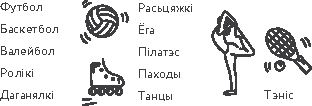
\includegraphics[scale=1.5]{willpower/ch5/11.pdf}\\
  \medskip
  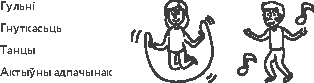
\includegraphics[scale=1.5]{willpower/ch5/12.pdf}
\end{figure}

\emph{Гульнявыя віды актыўнасьці зь іншымі людзьмі аказваюцца прыкметна больш карыснымі, чым адзіночныя віды спорту, з~пункту гледжаньня доўгатэрміновай пэрспэктывы. Мацней за ўсё падаўжаюць жыцьцё гульні з~ракеткай~--- такія як бадмінтон, тэніс і сквош. Аматары тэнісу жывуць на 9,7 гадоў даўжэй, бадмінтону~--- на 6,2, футболу~--- на 5, ровару~--- на 3,7, плыўцы жывуць на 3,4 гады даўжэй, чым тыя, хто грэбуе фізычнымі практыкаваньнямі.}

Галоўнае~--- ня трэба занадта старацца, хай гульня расслабляе вас. Як было заўважана: «Ніхто ня ставіцца да гульні ў~тэніс так сур'ёзна, як аматары, якія гуляюць па выходных». Гульні паглынаюць вашу ўвагу, даюць адпачынак ад стрэсу, расслабляюць, даюць магчымасьць камунікаваць, канкураваць і перамагаць. Няважна, якая гульня, ад тэнісу да Pokemon go, важныя задавальненьне і сумесны рух. Асабліва патрэбная спантанная актыўнасьць тым, хто знаходзіцца ў~дэпрэсіі ці выгараньні. 

\infobox{Гульні можна прыдумаць на пустым месцы, напрыклад хто саб'е каменем пустую бутэльку на лецішчы, хто далей закіне камень у~возера і да т.~п.}

Здаровы чалавек заўсёды мае патрэбу ў~руху. Зьніжэньне рухальнай актыўнасьці~--- гэта індыкатар перавышэньня фізычных або стрэсавых нагрузак. Як апэтыт прыходзіць падчас яды, так і задавальненьне ад руху прыходзіць падчас гульняў. Успомніце, як часта бывала, што вы не хацелі выбірацца на заняткі ці ў~парк, а, выбраўшыся, атрымлівалі задавальненьне ад руху і былі радыя прынятаму рашэньню.

\infobox{Атрымлівайце задавальненьне.} Многія людзі пазьбягаюць і баяцца фізычных практыкаваньняў, таму што для іх гэта цяжкая, нецікавая і руцінная праца. Але ж гэта ня так! Добрая кампанія, цікавы маршрут, новыя адкрыцьці зробяць вашу трэніроўку вясёлай, драйвовай і энэргічнай. Падыходзьце творча да свайго паўсядзённага раскладу: падумайце, дзе можна дадаць крыху актыўнасьці. Сумесная фізычная актыўнасьць зь сям'ёй ці сябрамі спрыяе ўзмацненьню матывацыі. Ня стойце на месцы падчас прагулкі з~сабакам, а~рухайцеся і гуляйце зь ім, як у~дзяцінстве.

\textbf{Чым больш вы рухаецеся, тым больш вам хочацца рухацца!}

Свой дом можна зрабіць куды больш рухомым, разьмясьціўшы розныя снарады і прыстасаваньні, якія стымулююць вас даўжэй рухацца: гіры, гантэлі, турнік, швэдзкую сьценку, балянсборды, слэклайн. Павесьце карціну ці фота зь людзьмі ў~руху~--- такія выявы падштурхоўваюць і нас больш рухацца. А калі вы заведзяце сабаку, то гэта таксама аўтаматычна павялічыць і ваш узровень актыўнасьці. Выбіраючы дом ці кватэру, поруч зь якой ёсьць парк ці прыгожыя сьцежкі-дарожкі, вы будзеце часьцей на іх гуляць.

Танцаваць можна дома, падчас гатаваньня ці ўборкі, і ў~дУшы, і ў~душЫ. Нават такі сур'ёзны таварыш, як Ніцшэ, пісаў: «Дзень прайшоў дарма, калі я не танцаваў». Танец мае наймагутнейшы антыстрэсавы эфэкт, і ўсё чалавецтва з~самых старажытных часоў танцавала і цешылася. Любую праблему на сьвеце можна вырашыць танцуючы!

\subsection*{Пытаньні і заданьні}

1. Пры якой фізычнай актыўнасьці вы можаце яшчэ і актыўна камунікаваць зь сябрамі?

2. Шукаеце, якую нагрузку дадаць? Няхай гэта будуць гульні або танцы!

3. Паглядзіце на вуліцу як на спартзалю: якія практыкаваньні на турніках, на зямлі, на дрэвах, з~уласнай вагой вы можаце прыдумаць?


\section{Рэжым фізычнае актыўнасьці}

Старажытнагрэцкі атлет Мілён Кратонскі штодня трэніраваўся, узвальваючы на плечы бычка і абыходзячы па коле гарадзкія сьцены. Па меры таго, як бычок рос, расла і сіла Мілёна. Так, прынцып паступовага павелічэньня нагрузкі й рэгулярнасьці вядомы яшчэ з~антычных часоў.

Для прагрэсу і кантролю здаровы рэжым фізычнае актыўнасьці трэба плянаваць па тыднях і разьлічваць сумарную тыднёвую нагрузку. Многія людзі лічаць, што можна сядзець цэлы дзень і затым усё гэта кампэнсаваць трэніроўкай ці яшчэ радыкальней~--- кампэнсаваць тыдзень сядзеньня ў~офісе трэніроўкай у~выходныя. Вядома, любая актыўнасьць лепшая, чым яе адсутнасьць, аднак карысьнейшыя кароткія падыходы, раўнамерна разьмеркаваныя на працягу дня, ад ранішняй зарадкі да вечаровага шпацыру.

\textbf{Улічваем усё:}
\begin{itemize}
  \item від і частасьць трэніровак; 
  \item павелічэньне нагрузкі; 
  \item цыкляваньне трэніровак або хвалевую пэрыядызацыю; 
  \item разнастайнасьць відаў нагрузкі і ўмоваў; 
  \item пункт супэркампэнсацыі, калі вашыя сілы цалкам аднавіліся пасьля трэніроўкі;
  \item адэкватнасьць аднаўленьня.
\end{itemize}

Калі вы берацеся за фізычныя трэніроўкі ўпершыню ці пасьля доўгага перапынку, то вам варта пачынаць, паступова павялічваючы аб'ём і нагрузку, і толькі адно пасьля таго, як колькасьць трэніровак і іх працягласьць адпрацаваныя, пераходзіць да нарошчваньня інтэнсіўнасьці нагрузкі. Працяглая аднолькавая праграма паступова вядзе да зьніжэньня вынікаў, таму для цяглічнага росту важна мяняць іх, шакаваць цягліцы, каб яны расьлі. 

\textbf{Памятайце, што рэжым у~здароўі~--- гэта самае істотнае для доўгатэрміновых вынікаў.} Занадта працяглыя перапынкі паміж трэніроўкамі могуць заўважна запаволіць прагрэс, пры гэтым у~дні стрэсу і дэдлайнаў, пры фастынгу важна палягчаць нагрузку да мінімальнай.

Прыкметамі \textbf{недатрэніраванасьці} зьяўляецца адсутнасьць росту паказьнікаў, а~\textbf{ператрэніраванасьць} выяўляецца ў~парушэньнях псыхаэмацыйнага стану, млявасьці, павышэньні пульсу або ціску ў~спакоі, цяглічных болях, пагаршэньні спартыўных вынікаў, парушэньнях сну, разьбітасьці на наступны дзень пасьля трэніроўкі, зьніжэньні імунітэту і страце матывацыі. Часта ператрэніраванасьць бывае ў~тых, хто спрабуе «кампэнсаваць» прапушчаную трэніроўку або паскорыць свой прагрэс занадта высокім прыростам нагрузкі~--- ня варта так рабіць! Для прафіляктыкі ператрэніраванасьці не падразайце свой каляраж, дзяліце праграму на блёкі, аднаўляйцеся ў~саўне і на масажы, пазьбягайце нутрыцэўтычных дэфіцытаў (мінэралы, вітаміны), рабіце перапынкі або памяншайце трэніровачны аб'ём пры прыкметах ператрэніраванасьці.

\subsection*{Адсочвайце прагрэс}

Прагрэс можна адсочваць: па крокамеры, па кілямэтрах бегу, па колькасьці паднятае вагі ці колькасьці падыходаў да турніка. Можна паставіць сабе плян у~100 ці больш прысяданьняў і гнутка разьмеркаваць іх на працягу дня, выпрацоўваючы свой плян да вечара,~--- выбірайце тое, што спрацуе для вас лепш. 

\infobox{Дзёньнік трэніровак, дзе вы адзначаеце сваё самаадчуваньне і робіце нататкі да тэхнікі,~--- ідэальнае рашэньне.}

\emph{Сучасныя рэкамэндацыі па фізычнай актыўнасьці гавораць, што дарослыя павінны аддаваць ня менш як 150 хвілінаў на тыдзень трэніроўкам сярэдняй інтэнсіўнасьці або ня менш як 75 хвілінаў высокай інтэнсіўнасьці, кожная трэніроўка павінна займаць ня менш як 10 хвілін. Для дадатковых перавагаў~--- адпаведна 300 хвілінаў сярэдняй і 150 хвілінаў высокай інтэнсіўнасьці. Сілавым практыкаваньням трэба аддаваць два і больш дзён на тыдзень. Аднак і гэтыя значэньні не дацягваюць да оптымуму нагрузкі.}

\subsection*{Лепей зусім мала, чым нічога}

Карысьць могуць прынесьці самыя кароткія эпізоды актыўнасьці: напрыклад, для станоўчага псыхалягічнага эфэкту часта дастаткова ўсяго 5--10 хвілінаў, а~вось трэніроўкі больш за 45--60 хвілінаў лепш не рабіць, замяніце працягласьць павелічэньнем іх частасьці. Розныя дасьледаваньні паказваюць, што пры хадзьбе працягласьцю 1--2 гадзіны на тыдзень (то бок па 15--20 хвілінаў на дзень) зьніжаецца імавернасьць інфаркту, інсульту і разьвіцьця дыябэту, памяншаецца рызыка заўчаснай сьмерці.

Дасьледаваньні паказалі, што нават адной высокаінтэнсіўнай інтэрвальнай трэніроўкі на тыдзень дастаткова, каб атрымаць паляпшэньне фізычнае формы, зьніжэньне ціску і паляпшэньне структуры цела. Пры гэтым адна такая трэніроўка мала чым саступае тром сярэднеінтэнсіўным трэніроўкам на тыдзень.

\subsection*{Прасьцей, яшчэ прасьцей} Калі ў~вас мала часу, то выкарыстоўвайце простыя падыходы, напрыклад абярыце 2--3 ключавых практыкаваньні і рабіце іх кожны дзень. А каб уцягнуцца, можаце пачаць і з~аднаго практыкаваньня ў~некалькі падыходаў. Калі ў~вас нестабільны графік і вам не ўдаецца вылучаць фіксаваны час для трэніровак, задайце сабе штотыднёвы аб'ём прысяданьняў, падцягваньняў, адцісканьняў, павесьце аркушык-сьпіс і рэгулярна на працягу дня выконвайце свой плян. Скажам, вы можаце пачаць з~адцісканьняў, прысяданьняў і падцягваньняў~--- і гэтага мінімуму вам можа быць дастаткова для пачатку.

\subsection*{Сумарная актыўнасьць}

А як падлічыць агульны ўзровень неабходнай актыўнасьці, калі я займаюся рознымі яе відамі? Бо карысна раўнамерна разьмяркоўваць яе віды: пагуляць у~парку, прабегчыся, падняць цяжкасьці. Існуе такі паказьнік, як мэтабалічны эквівалент (Metabolic Equivalents, METs),~--- гэта адзінка вымярэньня фізычнай нагрузкі, якая паказвае стаўленьне ўзроўню мэтабалізму падчас актыўнасьці да ўзроўню мэтабалізму ў~спакоі. Гэта значыць, што калі вы хутка ідзяце пешшу, то вашая актыўнасьць 4 MET, г.~зн. вы вытрачаеце ў~4 разы больш энэргіі, чым лежачы. Адна адзінка МЕТ прыблізна роўная 3,5 мл кіслароду на кіляграм вагі ў~хвіліну. Для прыкладу, праца за кампутарам 3, тэніс 5, баскетбол 8, бег 10 МЕТ.

Напрыклад, стандартная рэкамэндацыя ў~150 хвілінаў аэробных сярэднеінтэнсіўных практыкаваньняў (вышэй за 3 MET) або 75 хвілінаў бегу эквівалентная 450 MET-хвілінаў або 7,5 МЕТ-гадзінаў на тыдзень. Такая актыўнасьць памяншае сьмяротнасьць на 20\,\% у~параўнаньні з~тымі, хто ўвогуле не займаецца. Аднак аптымальная актыўнасьць будзе вышэйшай, пачынаючы з~900 МЕТ-хвілінаў або 15 МЕТ-гадзінаў да 20 МЕТ-гадзінаў. Так, жанчыны з~актыўнасьцю 21 MET гадзіна на тыдзень маюць рызыку раку грудзей у~2 разы менш, чым 2 МЕТ-гадзіны. Трэніруючыся з~інтэнсіўнасьцю паміж 22--75 MET, мы можам зьнізіць рызыку сьмерці на 40\,\%, а~вось большыя лічбы ўжо зьвязаныя з~павышэньнем рызыкі. Выкарыстоўваючы табліцы МЕТ значэньняў, вы можаце ацаніць свой тыднёвы ўзровень актыўнасьці.

\subsection*{Пытаньні і заданьні}

1. Ці адсочваеце вы свой прагрэс у~трэніроўках? Вядзеньне дзёньніка трэніровак дапаможа вам паскорыць свой прагрэс.

2. Ці прытрымліваецеся вы рэжыму трэніровак?

3. Як у~вас праяўляецца неда- і ператрэніраванасьць?


\section{Бяз скрайнасьцяў}

Мы, людзі,~--- істоты, схільныя да скрайнасьцяў: можам наносіць сабе шкоду ня толькі гіпадынаміяй, але й залішняй фізычнай актыўнасьцю. Навукоўцы высьветлілі, што прынцып «чым больш, тым лепш» у~трэніровачным працэсе не працуе, графік рух / карысьць мае U-падобную форму, то бок оптымум карысьнейшы за максімум.

Як гэта бывае? Чалавек прыходзіць у~фітнэс-клуб па спорт і здароўе, і, пад узьдзеяньнем спэцыфічнага асяродзьдзя, паступова пераходзіць на стэроіды, прэпараты для спальваньня тлушчу і да т.~п. У такіх месцах шмат людзей з~парушаным вобразам цела, таму могуць паўстаць, напрыклад, такія нездаровыя памкненьні, як спроба максімальнага зьніжэньня падскурнага тлушчу, што чэравата гарманальнымі праблемамі, асабліва ў~жанчынаў. У мужчынаў узьнікае бигорексия, або цяглічная дысмарфафобія,~--- гэта як анарэксія, толькі наадварот: жаданьне любой цаной набраць больш масы суправаджаецца пераяданьнем і фіксацыяй на трэніроўках.

\emph{Зьвярніце ўвагу, што залішняе спажываньне бялку, а~асабліва комплексаў амінакіслотаў ВСАА можа скарачаць працягласьць жыцьця і неспрыяльна ўзьдзейнічаць на мэтабалізм.}

\subsection*{Фітнэс-адыкцыя}

Заняткі спортам спрыяюць павышэньню настрою, таму ў~людзей, схільных да залежных паводзінаў, можа разьвіцца і фітнэс-адыкцыя~--- залежнасьць ад фізычнае актыўнасьці. У гэтым выпадку самаацэнка прывязваецца да спартовых посьпехаў і патрабуе нарошчваньня «дозы» і публічнага прызнаньня. 

\infobox{Калі чалавек займаецца спортам дзеля эўфарыі, павялічвае час заняткаў, у~выпадку пропуску ў~яго пагаршаецца настрой, ён выпадае з~сацыяльнага жыцьця і больш займаецца адзін, ці ігнаруе траўмы і боль,~--- гэта можна назваць залежнасьцю.}

Шматгадзінныя маратоны, бег з~высокім пульсам, злоўжываньне спрынтамі і сілавымі відамі спорту, уключаючы красфіт, можа павысіць рызыку арытмій, прыводзіць да небясьпечных для сэрца зьменаў, уключаючы гіпэртрафію і фіброз сэрца. Умераны бег можа падоўжыць жыцьцё на 6 гадоў, а~цяжкая атлетыка~--- усяго на паўтара года. 

Траўматычныя віды спорту, такія як рэгбі або бокс, павялічваюць рызыку посттраўматычнай дэмэнцыі. Удары па галаве багатыя ўскладненьнямі праз шмат гадоў, беражыце сваю галаву зь дзяцінства!

Часам у~пагоні за гострымі адчуваньнямі чалавек выбірае экстрэмальныя віды спорту, дзе вялікая рызыка траўмы, і са здароўем тут таксама мала агульнага. Небясьпечным зьяўляецца і рэзкі пачатак заняткаў любым спортам~--- важна заўсёды дзейнічаць паступова. Калі вы бегаеце, вывучыце тэхніку бегу, купіце адпаведны абутак, купіце пульсамер і датрымлівайцеся правільнага пульсавага рэжыму. У цяжкай атлетыцы вучыцеся правільна разьлічваць вагу і заўсёды старанна вывучайце тэхніку практыкаваньняў. Калі ня ўпэўненыя~--- зьвярніцеся да трэнера ў~пачатку заняткаў.

\textbf{Плянуйце свой трэніровачны графік, пазьбягаючы як ператрэніраванасьці, так і занадта рэдкіх заняткаў.}

\subsection*{Пытаньні і заданьні}

1. Ад чаго залежаць вашыя мэты ў~фізычнай актыўнасьці? Які вы бачыце сваю ідэальную форму?

2. Ці часта вы атрымліваеце спартыўныя траўмы? Ці можна іх пазьбегнуць?

3. Ці схільныя вы да фітнэс-адыкцыі?


\section{Цягліцы}

Існуе лекарскі анекдот, маўляў, пра жыцьцёвыя прыярытэты чалавека як віду можна сказаць па яго цягліцах, бо самая моцная~--- сківічная, а~самая вялікая~--- ягадзічная. Насамрэч колькасьць цяглічнай масы і яе функцыянальная актыўнасьць~--- важны рэсурс здароўя. Цягліцы зьяўляюцца магутнай абаронай мэтабалізму, зьніжаюць рызыку атлусьценьня і цукровага дыябэту, павялічваюць адчувальнасьць да інсуліну і абараняюць ад скокаў глюкозы і тлушчаў у~крыві. Мацнейшыя цягліцы павялічваюць працягласьць жыцьця, зьмяншаюць рызыку мноства захворваньняў, ад сардэчна-сасудзістых да анкалягічных. 

\textbf{З узростам колькасьць цягліцаў зьмяншаецца, яны замяшчаюцца тлушчам, сілавыя паказьнікі і трывушчасьць становяцца меншымі, але гэты працэс можа быць перадухілены трэніроўкамі.}

\emph{Мармуровае мяса.} Вы пэўна ж ведаеце пра гэты далікатэс і нават, магчыма, яго каштавалі. 

\emph{Гісторыя паходжаньня гэтага прадукту, які родам зь Японіі, паказальная і павучальная: перасечаная мясцовасьць, большасьць роўных участкаў засяваецца рысам, жывёлам няма дзе рухацца, таму яны большую частку часу праводзяць у~стойлах, дзе іх кормяць збожжам, а~не травой. Акрамя таго, у~іх рацыён уключаюць піва і сакэ. Падгадаваных жывёлаў падвешваюць на лейцах, каб яны не маглі рухацца, але й не ляжалі. Як вынік, мяса гэтых жывёлаў зьмяшчае нутрыцяглічны тлушч~--- так атрымліваецца «мармуровае мяса». Калі жывёла есьць траву і свабодна рухаецца, яго мяса ніколі не будзе такім тлустым.}

Нічога не нагадвае? Тое ж самае робяць людзі самі з~сабой спалучэньнем нерухомасьці з~ужываньнем збожжавых і алькагольных прадуктаў. \textbf{Гіпадынамія + высокавугляводнае харчаваньне + алькаголь = хуткая страта цяглічнай масы і адначасовае павелічэньне міжцяглічнага тлушчу.}

Пры гэтым працэс напачатку праходзіць неўпрыкметаў, бо аб'ёмы рук і ног могуць заставацца ранейшымі, а~вы толькі адчуваеце цяглічную слабасьць і згрыбеласьць. Саркапэнія, або страта цяглічнай масы, вельмі часта спалучаецца з~атлусьценьнем, і тады выкарыстоўваюць тэрмін «саркапэнічнае атлусьценьне». Гэта нядзіўна, бо клеткі-папярэднікі ў~цяглічнай і тлушчавай тканках агульныя.

Чым мацней падаюць сілавыя вынікі, тым менш у~вас цяглічнай масы, а~бывае і зваротная сытуацыя: вы павялічылі сілавую нагрузку, але ахоп канцавінаў раптам паменшыўся. Не сьпяшайцеся панікаваць: зьніжэньне аб'ёму зьвязанае не са стратай цягліцаў, а~з памяншэньнем міжцяглічнага тлушчу. Чым больш міжцяглічнага тлушчу, тым больш друзлым выглядае цела чалавека, бо тлушч, у~адрозьненьне ад цягліцаў, вісіць, бо ня мае тонусу.

Людзі пачынаюць «губляць» цягліцы вельмі рана: пры недастатковай фізычнай актыўнасьці пасьля 30 гадоў за кожныя 10 гадоў можа губляцца ад 3 да 5\,\% цяглічнай масы. У сярэднім да 50 гадоў губляецца каля 10\,\% і да 80~--- яшчэ 30\,\%. Узроставае зьніжэньне сілы складае 20--40 працэнтаў у~пажылых у~параўнаньні з~маладымі. Акрамя зьніжэньня фізычнай актыўнасьці важным чыньнікам рызыкі саркапэніі зьяўляецца зьніжэньне тэстастэрону і нізкае спажываньне бялку~--- для прафіляктыкі рэкамэндуецца павялічыць да 1,2--1,5 г на 1 кг вашай масы на дзень.

\emph{Павелічэньне сілы і цяглічнай масы з~дапамогай трэніровак дасягалася нават людзьмі ва ўзросьце 90+. Адзін год трэніровак можа аднавіць 30\,\% страчанай сілы ў~пажылых людзей, якую яны страчвалі на працягу апошніх 12 гадоў. Сілавыя трэніроўкі ў~пажылых на працягу паўгода паказваюць амаладжэньне цягліцаў на клеткавым узроўні аж да 30-гадовага стану.}

\textbf{Саркапэнія}~--- важны чыньнік рызыкі іншых хваробаў: астэапароз, дыябэт, сардэчна-сасудзістыя і іншыя захворваньні. Трэніроўкі зьніжаюць узровень запаленчых цытакінаў, нармалізуюць ціск, павышаюць адчувальнасьць да інсуліну, паляпшаюць гарманальны профіль, дапамагаюць падтрымліваць здароўе костак. Менавіта сілавыя трэніроўкі зьяўляюцца самым эфэктыўным відам фізычнае трэніроўкі для лячэньня саркапэніі. Іншыя віды актыўнасьці, такія як бег, хоць і павялічваюць цяглічную масу, але павольней і ў~меншым аб'ёме.

\subsection*{Пытаньні і заданьні}

1. Да якога паверха вы падымаецца бяз дыхавіцы?

2. Калі вы глядзіце на сябе ў~люстэрка, ці падабаецца вам, у~якой вы форме?

3. Як зьмянілася вашыя сіла і трывушчасьць за апошнія 3 гады?


\section{Цяглічная маса, сіла і функцыя}

Існуе мноства спосабаў вымярэньня цяглічнай масы, сілы і функцыі. Разгледзім некалькі зь іх. Так, гэта ўжо згаданыя намі DEXA, біяімпэданс і антрапамэтрычныя мэтады, якія вы можаце выкарыстоўваць самі.

\subsection*{Абхоп пляча}

Вымерайце мернай стужкай абхоп сярэдзіны пляча. Затым вазьміце пальцамі скуру пляча ў~складку і вымерайце яе таўшчыню з~дапамогай лінаркі. Паўтарыце вымярэньне, дамогшыся падобных значэньняў. 

Абхоп пляча (біцэпс) = акружнасьць~--- (3,14 x таўшчыня зморшчыны). Нізкія значэньні абхопу пляча зьвязаныя з~больш высокай рызыкай сьмяротнасьці, горшым мэнтальным здароўем і якасьцю жыцьця.

\textbf{Значэньні:} 

Норма: больш за 28 см (мужчыны), 23 см (жанчыны). 

Крытычныя значэньні: менш за 23 см (мужчыны) і 18 см (жанчыны). 

Прамежкавыя значэньні~--- ніжэйшыя паказьнікі.

\subsection*{Колькасьць адцісканьняў, прысяданьняў}

Маніторынг сваіх сілавых паказьнікаў~--- колькасьці адцісканьняў, прысяданьняў, падцягваньняў, як агульны лік, так і колькасьць за адну хвіліну, узьнятая вага і інш.~--- добры спосаб адзнакі стану цяглічнай сыстэмы. 

\textbf{Тыя мужчыны, якія змаглі адціснуцца за хвіліну больш за 40 разоў, мелі прыкметна меншую рызыку сардэчна-сасудзістых захворваньняў, чым тыя, хто адціскаўся менш за 10. Падлічыце, колькі разоў вы можаце падцягнуцца, прысесьці і адціснуцца за адзін падыход, запішыце гэтыя значэньні.}

\subsection*{Хуткасьць хадзьбы}

Чым хутчэй вы ходзіце, тым вышэйшы паказьнік здароўя. З дапамогай смартфона падлічыце сваю хуткасьць хадзьбы. Хуткасьць ніжэйшая за 2,16 км у~гадзіну зьвязаная з~самай высокай рызыкай. Чым вышэйшая хуткасьць, тым лепшыя паказьнікі для здароўя. 

\textbf{Аптымальная хуткасьць~--- больш за 4,3 км за гадзіну.}

\subsection*{Сіла сьціску ручыцы}

Вымяраецца з~дапамогай адмысловага дынамометра. Ня ведаю, як у~вас, але ў~мяне млявы поціск рук выклікае непрыемныя асацыяцыі. Цікава, што за апошнія дзесяцігоддзі поціск рукі мужчынаў стаў слабейшым, а~ў жанчынаў, наадварот, мацнейшым. Дасьледаваньні паказваюць, што сьмяротнасьць ад сардэчна-сасудзістых, лёгачных захворваньняў, інсультаў і шэрагу відаў раку зьвязаная са зьмяншэньнем сілы сьціску. Больш высокія значэньні~--- характарыстыка павышэньня даўгалецьця і зьніжэньня рызыкі многіх захворваньняў.

\textbf{Для мужчынаў} аптымальныя значэньні -- вышэй за 60 кг, норма~--- 45--60 кг. 

\textbf{Для жанчынаў} аптымальныя значэньні -- вышэй за 45 кг, норма~--- 25--45 кг. 

Больш дакладныя значэньні можна атрымаць, калі суаднесьці сілу з~масай цела. Сілу падзяліць на масу цела і памножыць на 100: у~мужчынаў сярэднія значэньня складаюць 60--70\,\% масы цела, у~жанчынаў~--- 45--50\,\%.

\subsection*{Планка}

Прыміце ўпор лежачы на локцях. Засячыце час, на працягу якога вы можаце ўтрымліваць гэтую позу. Таксама можна рабіць бакавыя планкі (правую і левую). Аптымальна: больш за 180 сэкундаў. Нармальна: 100--180 сэкундаў.

\subsection*{Тэст на балянс}

Пакладзіце рукі на пояс. Падніміце адну нагу і ўпрыце яе ступаком у~процілеглую нагу на ўзроўні калена. 

Засячыце час да страты раўнавагі або зрушэньня апорнай нагі: аптымальна~--- больш за 60 сэкундаў, нармальна~--- 40--60 сэкундаў. 

Заплюшчыце вочы і зрабіце тое ж самае: аптымальна~--- больш за 27 сэкундаў, нармальна~--- 15--27 сэкундаў.

\subsection*{Тэсты на скачкі}

Павесьце мерную стужку на сьцяну, адмераўшы два мэтры ад падлогі. Зафіксуйце кропку, да якой вы дацягваецеся рукой. Затым скокніце ў~вышыню, імкнучыся дасягнуць найболей высокай кропкі, выніковы вынік лічыцца як розьніца паміж кропкамі. Паспрабуйце некалькі разоў, абярыце лепшы вынік: норма~--- 40--50 см, выдатны вынік~--- больш за паўмэтра. Скачкі ў~даўжыню: сагніце ногі ў~каленях і скокніце наперад, дапамагаючы сабе махам рукамі. Норма~--- больш за 2 м 10 см, выдатны вынік~--- звыш 2 м 40 см.

\subsection*{Пытаньні і заданьні}

1. Які ў~вас ахоп біцэпса?

2. Вымерайце сілу ручыцы дынамометрам.

3. Колькі разоў вы можаце прысесьці, падцягнуцца, адціснуцца?


\section{Кардыярэсьпіраторныя тэсты}

Нагрузачныя тэсты вельмі эфэктыўныя для выяўленьня схаваных паталягічных працэсаў у~арганізьме. Хуткасьць адхіленьня функцый пры нагрузцы і хуткасьць іх узнаўленьня зьяўляюцца інфарматыўнымі спосабамі ацэнкі рэзэрву функцыі і рэзэрву рэгуляцыі. Як той казаў, «дзе коратка~--- там і рвецца», таму такая ацэнка зьніжэньня рэзэрву і павышэньня, у~шырокім сэнсе, «крохкасьці» вельмі карысная для прафіляктыкі здароўя.

Стан сардэчна-сасудзістай і дыхальнай сыстэмаў~--- гэта найважнейшы паказьнік нашага здароўя і біялягічнага ўзросту. Іх больш высокія рэсурсы забясьпечваюць ня толькі лепшую фізычную форму і пераноснасьць нагрузак, але й даўгалецьце, а~таксама зьніжэньне рызыкі розных захворваньняў. Чым вышэйшыя гэтыя рэсурсы, тым вышэйшыя вашыя кагнітыўныя здольнасьці, стрэсаўстойлівасьць, узровень энэргіі і многае іншае. 

\textbf{Трэніроўкі могуць палепшыць рэсурсы сардэчна-са\-су\-дзіс\-тай і цяглічнай сыстэмаў нават у~самым сталым узросьце.}

\subsection*{Артастатычная проба}

Ацэньвае стан сардэчна-сасудзістай сыстэмы. Вызначыце ваш пульс лежачы. Устаньце і праз тры хвіліны памерайце пульс яшчэ раз. Унясіце абодва значэньні. 

\textbf{Розьніца ў~ЧСС:} ня больш за 11 удараў~--- оптымум (чым менш, тым лепш), 12--18~--- норма, больш за 19~--- зьніжана.

\subsection*{Затрымка дыханьня}

Затрымка дыханьня ацэньвае пераноснасьць гіпаксіі. Затрымайце дыханьне на поўным удыху, закрыўшы нос пальцамі. Значэньні: затрымка менш за 39 сэкундаў~--- паніжаны паказьнік, 40--49~--- норма, вышэй за 50~--- оптымум.

\subsection*{Проба Штанге}

Гэтая проба ацэньвае рэсурсы дыхальнай і сардэчна-сасудзістай сыстэмаў. Памерайце свой пульс стоячы. Затым сядзьце на крэсла, зрабіце тры ўдыхі, потым затрымайце дыханьне (нос закрыць пальцамі) на поўным удыху. Засячыце час, які вы можаце вытрымаць, і памерайце свой пульс адразу пасьля першага ўдыху. Падлічыце пульс за 30 сэкундаў (пасьля тэсту) і падзяліце на значэньне пульсу за 30 сэкундаў (да тэсту), выніковае значэньне не павінна перавышаць 1,2. Аптымальная пераноснасьць гіпаксіі~--- да 1,1, нармальная пераноснасьць гіпаксіі~--- да 1,2, дрэнная пераноснасьць гіпаксіі~--- вышэй за 1,2.

\subsection*{Проба Руф'е--Дыксана}

Ляжце на сьпіну, ляжыце на працягу 5 хвілінаў. Памерайце пульс за 15 сэкундаў (P1), затым на працягу 45 сэкундаў зрабіце 30 прысяданьняў. Пасьля гэтага кладзіцеся і пмерайце пульс за першыя 15 сэкундаў (P2). Праз 45 сэкундаў зноў памерайце пульс за 15 сэкундаў (P3). Унясіце значэньні ў~формулу: ((P2--70) + 2(P3-P1))/10. Падлічыўшы, вы атрымаеце значэньне індэкса. Значэньні 0,1--5 паказваюць аптымальную фізычную працаздольнасьць, 5,1--8~--- нармальную фізычную працаздольнасьць, больш за 8~--- нізкую.

\subsection*{Максімальнае спажываньне кіслароду (МСК, ViO\textsubscript{2}max)}

МСК~--- гэта максімальны ўзровень выкарыстаньня і дастаўкі кіслароду пры максімальнай нагрузцы, вымяраецца ў~мл / мін / кг і зьяўляецца адным з~самых важных маркераў здароўя. Нізкія кардыярэсьпіраторныя рэзэрвы вядуць да павелічэньня рызыкі заўчаснае сьмерці і павышэньня рызыкі захворваньняў. Павелічэньне МСК зьніжае рызыку праз аптымізацыю работы сэрца, лепшага кровазабесьпячэньня цягліцаў і росту капіляраў у~іх, паляпшэньня работы мітахондрыяў. 

\infobox{Па сутнасьці, ваш МСК~--- гэта паказьнік рэальнага біялягічнага, а~ня пашпартнага ўзросту, бо можна і ў~50 гадоў мець паказьнікі 25-гадовага.}

У нетрэніраваных людзей МСК зьніжаецца ўжо з~20 гадоў, прычым у~мужчынаў страта адбываецца з~хуткасьцю 0,5 мл / мін / кг, у~жанчынаў~--- 0,3 мл / мін / кг за год. Пры гэтым людзі ва ўзросьце 55--70 гадоў, якія чатыры месяцы актыўна займаліся хадзьбой альбо бегам, павысілі МСК: мужчыны~--- на 27\,\%, жанчыны~--- на 9\,\%. Тыя, хто займаецца спортам, маюць паказьнікі МСК, якія значна пераўзыходзяць звычайных людзей. Так, мужчына ва ўзросьце 30 гадоў можа мець МСК 40 мл/кг/мін, а~прафэсійны бягун~--- да 75 мл/кг/мін.

\textbf{Сярэднімі зьяўляюцца велічыні МСК: для мужчыны 52~--- (0,25 × узрост), для жанчыны 44~--- (0,20 × узрост).} 

\textbf{Мужчыны}: оптымум~--- 45 і вышэй, норма~--- 40--45, паніжаны паказьнік~--- 30--40, крытычны~--- менш за 30. 

\textbf{Жанчыны}: аптымальна~--- вышэй за 40, норма~--- 35--40, паніжаны паказьнік~--- 25--35, крытычны~--- ніжэй за 25.

Вымераць ViO\textsubscript{2}max дакладней за ўсё можна ў~лябараторыі. Менш дакладныя значэньні дае фітнэс-бранзалет. Вы можаце самі вымераць ViO\textsubscript{2}max у~тэсьце Купера. Для гэтага вам трэба прабегчы максімальна магчымую адлегласьць па роўнай мясцовасьці (стадыён зь вядомай акружнасьцю) за 12 хвілінаў. Унясіце адлегласьць, якую вы змаглі прабегчы, у~мэтрах. Разьлік па формуле: VO\textsubscript{2}max = (D\textsubscript{12} -- 504,9) / 44,73.

\subsection*{Пытаньні і заданьні}

1. Якія вашыя вынікі ў~артастатычнай пробе?

2. Падлічыце свае вынікі пробаў Штанге і Руф'е.

3. Памерайце свой МСК.

\clearpage
\thispagestyle{empty}
\begin{figure}[htb!]
  \vspace*{-0.25in}
  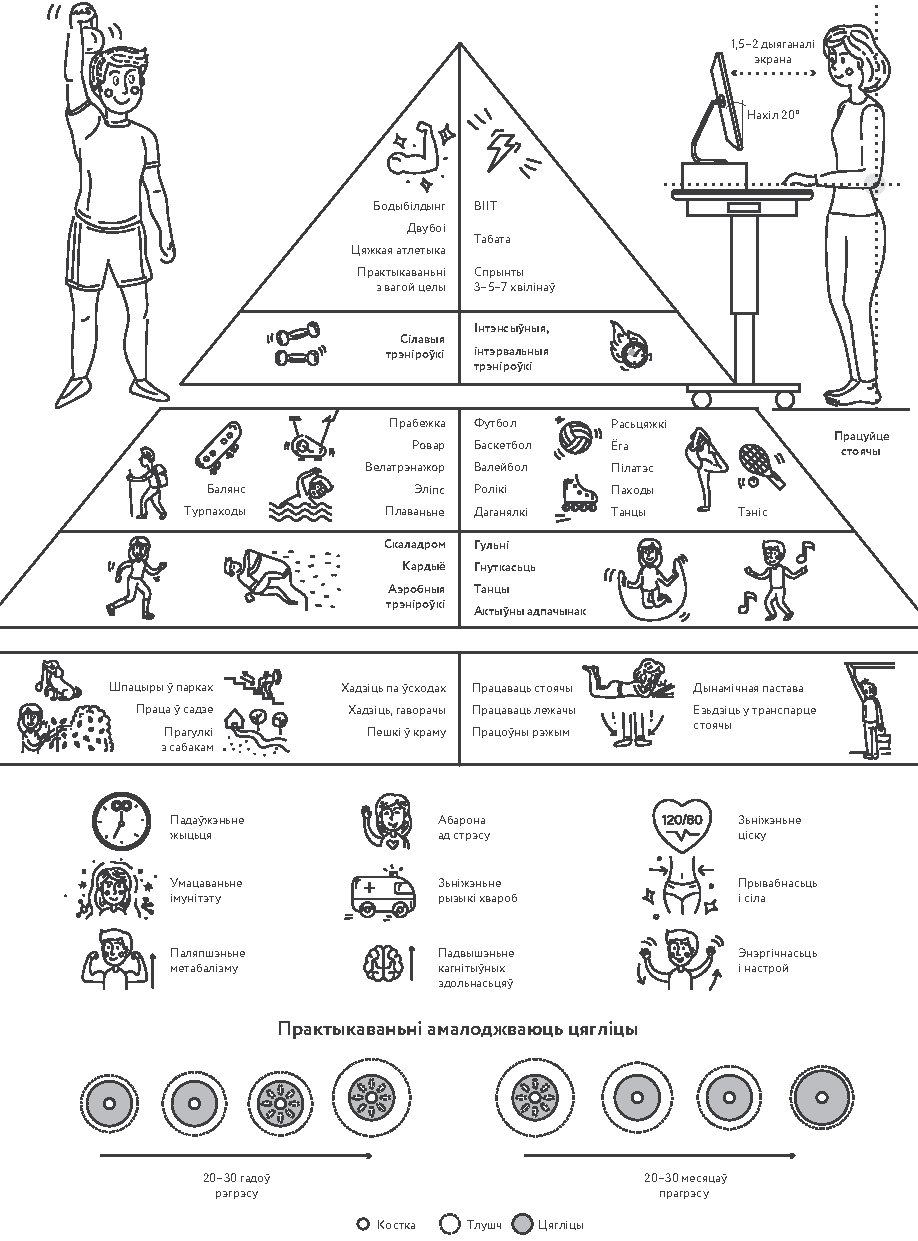
\includegraphics[width=\textwidth]{willpower/ch5/full.pdf}  
\end{figure}
